% !TeX program = xelatex
% Formal Chinese engineering report for the SAR16B self-calibration project.
% Build with XeLaTeX three times from this directory.
\documentclass[UTF8,fontset=none,a4paper,11pt,openany]{ctexrep}

\newcommand{\ReferenceReportTitle}{16 位 SAR 片上自校准与 SRM 行为验证}
\newcommand{\EvidenceCommit}{8e35335ed51fdd015be54ce4909c717dcb22509d}
\newcommand{\ToolboxCommit}{a8995cf4faf73dde9918589bfeb866c6a77db12d}

\usepackage[margin=2.25cm,headheight=14pt,headsep=10pt,footskip=18pt]{geometry}
\usepackage{fontspec}
\usepackage{xeCJK}
\XeTeXgenerateactualtext=1
\defaultfontfeatures{Ligatures=TeX}
\setmainfont{Latin Modern Roman}
\setsansfont{Latin Modern Sans}
\setmonofont{lmmono10-regular.otf}[
  BoldFont={lmmonolt10-bold.otf},
  ItalicFont={lmmono10-italic.otf},
  BoldItalicFont={lmmonolt10-boldoblique.otf}
]
\setCJKmainfont{FandolSong-Regular}[
  BoldFont={FandolSong-Bold},
  ItalicFont={FandolKai-Regular},
  BoldItalicFont={FandolSong-Bold}
]
\setCJKsansfont{FandolSong-Regular}[BoldFont={FandolSong-Bold}]
\setCJKmonofont{FandolSong-Regular}[BoldFont={FandolSong-Bold}]
\newCJKfontfamily\ReferenceCJKTitle{FandolSong-Bold}[BoldFont={FandolSong-Bold}]

\usepackage{amsmath,amssymb,mathtools,bm}
\usepackage{booktabs,tabularx,longtable,array,multirow}
\usepackage{graphicx,float}
\usepackage{xcolor}
\usepackage[most]{tcolorbox}
\usepackage{caption,subcaption}
\usepackage{enumitem}
\usepackage{fancyhdr}
\usepackage{titlesec}
\usepackage{needspace}
\usepackage{microtype}
\usepackage{listings}
\usepackage{xurl}
\usepackage{hyperref}
\usepackage{bookmark}

\newcolumntype{L}[1]{>{\raggedright\arraybackslash}p{#1}}
\newcolumntype{Y}{>{\raggedright\arraybackslash}X}

\definecolor{RefNavy}{HTML}{163A5F}
\definecolor{RefTeal}{HTML}{167C80}
\definecolor{RefGreen}{HTML}{288C3C}
\definecolor{RefOrange}{HTML}{D97706}
\definecolor{RefPurple}{HTML}{705B86}
\definecolor{RefGray}{HTML}{6B7280}
\definecolor{RefPaleBlue}{HTML}{EAF2F8}
\definecolor{RefPaleTeal}{HTML}{E8F5F4}
\definecolor{RefPaleGreen}{HTML}{E1F5E1}
\definecolor{RefPaleOrange}{HTML}{FFF3E0}
\definecolor{RefPalePurple}{HTML}{F2EDF7}
\definecolor{RefPaleGray}{HTML}{F3F4F6}

\setlength{\parindent}{2em}
\setlength{\parskip}{0pt}
\setlength{\emergencystretch}{2em}
\linespread{1.12}
\setlist{nosep,leftmargin=2em}
\renewcommand{\arraystretch}{1.22}
\captionsetup{font=small,labelfont=bf,justification=centering,singlelinecheck=true}

\titleformat{\chapter}[hang]
  {\centering\ReferenceCJKTitle\bfseries\fontsize{20.66}{30}\selectfont}
  {第\,\thechapter\,章}{1.4em}{}
\titlespacing*{\chapter}{0pt}{18pt}{34pt}
\titleformat{\section}
  {\Needspace{5\baselineskip}\centering\ReferenceCJKTitle\bfseries\fontsize{14.35}{22}\selectfont}
  {\thesection}{1em}{}
\titlespacing*{\section}{0pt}{21pt}{12pt}
\titleformat{\subsection}
  {\Needspace{4\baselineskip}\centering\ReferenceCJKTitle\bfseries\fontsize{12}{18}\selectfont}
  {\thesubsection}{0.8em}{}
\titlespacing*{\subsection}{0pt}{16pt}{8pt}
\titleformat{\subsubsection}
  {\Needspace{3\baselineskip}\ReferenceCJKTitle\bfseries\normalsize}
  {\thesubsubsection}{0.7em}{}

\pagestyle{fancy}
\fancyhf{}
\fancyhead[L]{\small\ReferenceReportTitle}
\fancyhead[R]{\small\nouppercase{\leftmark}}
\fancyfoot[C]{\small\thepage}
\renewcommand{\headrulewidth}{0.4pt}
\renewcommand{\footrulewidth}{0pt}
\fancypagestyle{plain}{
  \fancyhf{}
  \fancyfoot[C]{\small\thepage}
  \renewcommand{\headrulewidth}{0pt}
}

\newtcolorbox{methodbox}[1]{
  enhanced,breakable,sharp corners,boxrule=0pt,
  borderline west={1.4pt}{0pt}{RefNavy},
  colback=RefPaleBlue,colbacktitle=RefPaleBlue,coltitle=RefNavy,titlerule=0pt,
  left=7pt,right=7pt,top=5pt,bottom=6pt,
  fonttitle=\bfseries,title={#1},before skip=7pt,after skip=7pt
}
\newtcolorbox{evidencebox}[1]{
  enhanced,breakable,sharp corners,boxrule=0pt,
  borderline west={1.4pt}{0pt}{RefTeal},
  colback=RefPaleTeal,colbacktitle=RefPaleTeal,coltitle=RefTeal,titlerule=0pt,
  left=7pt,right=7pt,top=5pt,bottom=6pt,
  fonttitle=\bfseries,title={#1},before skip=7pt,after skip=7pt
}
\newtcolorbox{passbox}[1]{
  enhanced,breakable,sharp corners,boxrule=0pt,
  borderline west={1.4pt}{0pt}{RefGreen},
  colback=RefPaleGreen,colbacktitle=RefPaleGreen,coltitle=RefGreen,titlerule=0pt,
  left=7pt,right=7pt,top=5pt,bottom=6pt,
  fonttitle=\bfseries,title={#1},before skip=7pt,after skip=7pt
}
\newtcolorbox{riskbox}[1]{
  enhanced,breakable,sharp corners,boxrule=0pt,
  borderline west={1.4pt}{0pt}{RefOrange},
  colback=RefPaleOrange,colbacktitle=RefPaleOrange,coltitle=RefOrange,titlerule=0pt,
  left=7pt,right=7pt,top=5pt,bottom=6pt,
  fonttitle=\bfseries,title={#1},before skip=7pt,after skip=7pt
}
\newtcolorbox{diagnosticbox}[1]{
  enhanced,breakable,sharp corners,boxrule=0pt,
  borderline west={1.4pt}{0pt}{RefPurple},
  colback=RefPalePurple,colbacktitle=RefPalePurple,coltitle=RefPurple,titlerule=0pt,
  left=7pt,right=7pt,top=5pt,bottom=6pt,
  fonttitle=\bfseries,title={#1},before skip=7pt,after skip=7pt
}
\newtcolorbox{reproductionbox}[1]{
  enhanced,breakable,sharp corners,boxrule=0pt,
  borderline west={1.4pt}{0pt}{RefGray},
  colback=RefPaleGray,colbacktitle=RefPaleGray,coltitle=RefGray,titlerule=0pt,
  left=7pt,right=7pt,top=5pt,bottom=6pt,
  fonttitle=\bfseries,title={#1},before skip=7pt,after skip=7pt
}

\hypersetup{
  unicode=true,
  colorlinks=true,
  linkcolor=RefNavy,
  citecolor=RefTeal,
  urlcolor=RefPurple,
  pdftitle={16 位 SAR 片上前景自校准与 SRM 独立行为验证报告},
  pdfauthor={SAR ADC Digital Process Project},
  pdfsubject={Foreground self-calibration, Q8 reconstruction, SRM and ADCToolbox verification},
  pdfkeywords={SAR ADC, foreground calibration, SRM, Q8, INL, DNL, SNDR}
}
\urlstyle{same}
\setcounter{tocdepth}{2}
\setcounter{secnumdepth}{3}
\graphicspath{{../outputs/}}

\lstdefinestyle{projectcode}{
  basicstyle=\ttfamily\footnotesize,
  backgroundcolor=\color{RefPaleGray},
  frame=single,
  framerule=0.25pt,
  rulecolor=\color{RefGray},
  breaklines=true,
  breakatwhitespace=false,
  columns=fullflexible,
  keepspaces=true,
  showstringspaces=false,
  xleftmargin=5pt,
  xrightmargin=5pt,
  aboveskip=7pt,
  belowskip=7pt
}
\lstset{style=projectcode}

\newcommand{\metric}[1]{\textbf{#1}}
\newcommand{\statuspass}{\textcolor{RefGreen}{\textbf{PASS}}}
\newcommand{\statusgap}{\textcolor{RefOrange}{\textbf{GAP}}}
\newcommand{\statusnoclaim}{\textcolor{RefGray}{\textbf{NO CLAIM}}}

\begin{document}

% -----------------------------------------------------------------------------
% Cover
% -----------------------------------------------------------------------------
\begin{titlepage}
  \thispagestyle{empty}
  \centering
  \vspace*{2.25cm}
  {\ReferenceCJKTitle\bfseries\fontsize{17.22}{27}\selectfont
   16 位 SAR 片上前景自校准与 SRM\par}
  \vspace{0.35cm}
  {\ReferenceCJKTitle\bfseries\fontsize{17.22}{27}\selectfont
   独立行为验证报告\par}
  \vspace{0.55cm}
  {\large Physical-CDAC Mismatch, Q8 Reconstruction and Paired Noise Ablation\par}
  \vspace{0.9cm}
  {\color{RefNavy}\rule{0.25\textwidth}{1.1pt}\par}
  \vspace{1.3cm}
  \begin{tabular}{rl}
    \textbf{文档类型：} & 学术与工业维护联合报告\\
    \textbf{工程对象：} & SAR ADC Digital Process\\
    \textbf{算法对象：} & 16-bit on-chip foreground self-calibration\\
    \textbf{证据等级：} & 行为级闭环验证\\
    \textbf{冻结日期：} & 2026-08-30\\
    \textbf{证据提交：} & \texttt{\EvidenceCommit}\\
  \end{tabular}
  \vfill
  {\small
  本报告区分数字算法验证、mixed-signal 集成验证与硅片签核。\par
  报告中的行为级结果不得解释为 PEX、GDS 或实测硅片结论。\par}
  \vspace{1.0cm}
\end{titlepage}

\pagenumbering{Roman}

% -----------------------------------------------------------------------------
% Abstract and executive summary
% -----------------------------------------------------------------------------
\chapter*{摘要}
\addcontentsline{toc}{chapter}{摘要}

本报告对工程中的 16 位 SAR ADC 数字前景自校准、20 次冗余判决加权重构和 22-decision statistical residue measurement（SRM）进行了独立行为级复核。主算法不是外部正弦拟合，而是工程文件夹内的片上 P/N 递归校准：低 6 位作为参考 DAC，依次校准 bit6 至 bit19，每个目标位执行 32 组 P/N 测量，并对最高两位使用保护补偿；校准结果以 signed Q8 写回，随后由 RTL 等价重构路径生成 signed 16-bit 输出。

实验首先建立理想 16 位量化器控制组，得到 98.093 dB SNDR，与理论值 98.080 dB 相差 0.013 dB。随后在 normal-conversion 随机噪声关闭、同一 physical-CDAC mismatch realization 下隔离失配：未校准 SNDR 为 61.630 dB，片上自校准后为 93.433 dB，加入 expected-count SRM 后为 95.437 dB；INL 峰峰值由 108.505 LSB 降至 2.732 LSB，再降至 1.909 LSB，missing codes 由 1061 降至 4，再降至 0。片上校准的 gain-aligned weight RMSE 从 9.286 LSB 降至 0.2286 LSB，改善 40.63 倍。

为回答“SRM 是否真正降噪”，报告另设 32 次独立重复的成对带噪声消融。每次重复中 SRM on/off 共用完全相同的 noisy raw-bit stream，只改变 held-residue 的数字估计。对 project self-cal weights，22-decision SRM 将平均 SNDR 从 $89.716\pm0.059$ dB 提高到 $93.888\pm0.049$ dB，并将 affine-aligned error RMS 从 0.6722 LSB 降至 0.4158 LSB；对 oracle physical weights，相应 SNDR 增益为 $5.356\pm0.056$ dB。该结果证明当前行为边界内的 comparator/residue 路径存在明确降噪收益，但不复现 split-sampling、AZ aliasing 或论文完整的 $111\rightarrow38~\mu\mathrm{V}_{\mathrm{rms}}$ 晶体管噪声预算。

\begin{evidencebox}{核心结论}
在当前 6+4+5+5 physical-CDAC proxy、Q8 固定点契约与 RTL 等价行为模型下，工程中的 16 位片上前景自校准能够显著消除静态失配；SRM 也能在公平成对的带比较器噪声实验中降低剩余误差。尚未闭合的是 VCM 首次切换、真实 CDAC/comparator 时序、split-sampling 与 AZ 噪声机理、CDC/PHY 集成以及 ASIC physical signoff。
\end{evidencebox}

\noindent\textbf{关键词：}16 位 SAR ADC；片上前景自校准；P/N offset cancellation；Q8 固定点；SRM；CDAC 失配；SNDR；INL/DNL；ADCToolbox

\clearpage
\chapter*{执行摘要}
\addcontentsline{toc}{chapter}{执行摘要}

\begin{passbox}{已由可执行证据支持}
\begin{enumerate}
  \item 输出定义为 signed 16 bit；20 表示冗余判决数，不表示 20 位 ADC。
  \item 项目主算法确为片上 6-bit LSB-reference、P/N、32-pair、bit6--bit19 递归校准。
  \item 理想 16 位控制达到 98.093 dB，FFT 与 code-scale 基准正确。
  \item 同一失配样本中，self-cal only 提升 SNDR 31.804 dB；加 expected SRM 后总提升 33.807 dB。
  \item 公平成对带噪实验中，SRM on/off 原始 20-decision raw bits 完全相同，project self-cal 路径平均提升 4.172 dB。
  \item 五项本包测试通过；与既有行为模型联合回归共 21 项通过。
\end{enumerate}
\end{passbox}

\begin{riskbox}{不能由当前证据推出}
\begin{enumerate}
  \item 不能把行为模型结果写成 Huang 论文 93.7 dB 硅片实测复现。
  \item 不能把 SRM residue recovery 等同于完整 SS+SRM 噪声预算。
  \item 不能把 ADCToolbox 外部 sine-fit 当作片上校准 FSM。
  \item 不能据此宣称 VCM switching、comparator timing、PVT、PEX、DRC/LVS 或 silicon yield 已通过。
\end{enumerate}
\end{riskbox}

\begin{table}[H]
\centering
\caption{关键判定状态}
\label{tab:executive-status}
\begin{tabularx}{\textwidth}{>{\bfseries}p{0.27\textwidth}p{0.14\textwidth}X}
\toprule
判定对象 & 状态 & 证据摘要\\
\midrule
16 位定义与固定点契约 & \statuspass & signed 16-bit 输出；20 decisions；Q8 中 256 = 1 final-code LSB\\
片上 P/N 自校准身份 & \statuspass & 6-bit reference、14 targets、32 P/N pairs、最高两位保护\\
失配校准有效性 & \statuspass & SNDR $61.630\rightarrow93.433$ dB；gain-aligned RMSE 改善 40.63 倍\\
SRM 数字降噪行为 & \statuspass & 同 raw bits 下 self-cal 路径平均增益 $4.172\pm0.079$ dB\\
FPGA/ASIC 顶层集成 & \statusgap & adapter、CDC、mode arbitration、calibration PHY 尚未闭合\\
GDS 与硅片结论 & \statusnoclaim & 未执行 PnR、PEX、DRC/LVS、AMS 或硅片测试\\
\bottomrule
\end{tabularx}
\end{table}

\clearpage
\tableofcontents
\clearpage
\listoffigures
\clearpage
\listoftables
\clearpage
\pagenumbering{arabic}

% -----------------------------------------------------------------------------
\chapter{研究对象、范围与证据边界}

\section{首先澄清：这是 16 位片上自校准}

本项目的主对象不是 20 位 ADC，也不是 ADCToolbox 的外部拟合器。其真实层次关系为
\begin{equation}
\boxed{\begin{aligned}
\text{signed 16-bit output}
&\leftarrow 20\text{ redundant decisions}\\
&\leftarrow 20\text{ effective weights}\\
&\leftarrow 6\text{-bit reference calibrating 14 higher weights}
\end{aligned}}
\end{equation}
20 是冗余 SAR 的判决维数；16 才是最终有效输出宽度。多出的判决用于非二进制冗余、split-CDAC 以及误差恢复，不应被解释为额外输出位数。

\begin{methodbox}{工程内片上数据流}
低 6 位 reference section $\rightarrow$ target bit6 $\rightarrow$ P/N polarity search $\rightarrow$ 32-pair averaging $\rightarrow$ Q8 shadow-weight update $\rightarrow$ 逐位递归至 bit19 $\rightarrow$ b18/b19 protected search $\rightarrow$ synchronous writeback $\rightarrow$ normal 20-decision reconstruction $\rightarrow$ optional 22-decision SRM $\rightarrow$ signed 16-bit code。
\end{methodbox}

ADCToolbox 的 \texttt{calibrate\_weight\_sine()} 需要已知正弦激励和整段 raw-bit capture，通过浮点全局最小二乘识别权重。本报告仅将其作为 \texttt{ADCTOOLBOX\_SINE\_EXTERNAL\_BASELINE}。它不产生 RTL 所需的 \texttt{w\_wr\_en/w\_wr\_addr/w\_wr\_data} 时序，也不能替代 P/N FSM。

\section{证据分层}

\begin{table}[H]
\centering
\caption{本报告采用的证据分层}
\label{tab:evidence-levels}
\begin{tabularx}{\textwidth}{p{0.17\textwidth}p{0.23\textwidth}X}
\toprule
层级 & 本报告状态 & 可支持的结论\\
\midrule
L0 数学契约 & 已核对 & 位宽、Q8 单位、P/N 平均、SRM 概率模型和重构方程\\
L1 行为级模型 & 已运行 & 在给定 physical-CDAC proxy 与噪声条件下的算法有效性\\
L2 RTL 单元级 & 既有证据 & 三个核心 RTL 的 Vivado/XSIM 单元验证与综合可行性\\
L3 mixed-signal/AMS & 未完成 & 真实 VCM、CDAC switching、comparator timing 与噪声谱\\
L4 physical signoff & 未完成 & SDC/MMMC、CDC/RDC、LEC、DFT、PnR、DRC/LVS/PEX\\
L5 silicon & 未完成 & 实测 SNDR、噪声、功耗、良率与论文指标复现\\
\bottomrule
\end{tabularx}
\end{table}

\begin{diagnosticbox}{阅读规则}
报告中的 ``oracle'' 是行为模型内的数学上限；``expected SRM'' 是期望 count 的确定性上限；``stochastic SRM'' 才包含 22 次有限统计观察。三者均不是硅片测量。所有性能数字均应与其条件、decoder 和证据层级一起引用。
\end{diagnosticbox}

\section{文档与版本控制}

\begin{table}[H]
\centering
\caption{文档控制信息}
\label{tab:doc-control}
\begin{tabularx}{\textwidth}{>{\bfseries}p{0.25\textwidth}X}
\toprule
项目 & 内容\\
\midrule
工程根目录 & \path{D:/ReedZhao/Document/ADC_Digital_PROCESS/proc_vivado/sar_adc_v3}\\
Git 分支 & \texttt{main}\\
算法与实验冻结提交 & \texttt{\EvidenceCommit}\\
ADCToolbox 版本 & 0.9.1\\
ADCToolbox 审计提交 & \texttt{\ToolboxCommit}\\
报告日期 & 2026-08-30\\
证据等级 & 行为级验证，不是 AMS、PEX、GDS 或硅片签核\\
\bottomrule
\end{tabularx}
\end{table}

% -----------------------------------------------------------------------------
\chapter{工程组织与实现边界}

\section{独立行为实验包}

本次交付将实验编排置于独立目录，避免混入核心 RTL。项目算法本体继续复用工程中已存在、与 RTL 契约一致的行为模型。目录结构如下。

\begin{lstlisting}
analysis/self_cal_adctoolbox_behavioral_20260830/
|-- README.md
|-- requirements.txt
|-- THIRD_PARTY_NOTICES.md
|-- run_self_cal_behavioral.py
|-- test_self_cal_behavioral.py
|-- SELF_CAL_BEHAVIORAL_REPORT_CN.md
|-- reviews/
|   `-- REVIEW_01_ADCTOOLBOX_AUDIT_CN.md
|-- outputs/
|   |-- summary.json
|   |-- metrics.csv
|   |-- weights.csv
|   |-- srm_noise_ablation.csv
|   |-- calibration_trace.json
|   |-- run_log.txt
|   |-- fig_weight_error.png
|   |-- fig_spectrum_compare.png
|   |-- fig_inl_compare.png
|   |-- fig_calibration_trace.png
|   `-- fig_srm_noise_ablation.png
`-- report/
    `-- SAR16B_SELF_CAL_SRM_BEHAVIORAL_REPORT_CN.tex
\end{lstlisting}

\section{复用模块及其职责}

\begin{table}[H]
\centering
\small
\caption{行为实验复用的项目模块}
\label{tab:reused-modules}
\begin{tabularx}{\textwidth}{L{0.33\textwidth}Y}
\toprule
文件或模块 & 复用内容\\
\midrule
\path{analysis/full_sar_behavioral_20260729/full_sar_model.py} & P/N search、32-pair average、bit6--bit19 recursion、b18/b19 protection、20-decision conversion、SRM LUT 和 Q8 reconstruction\\
\path{analysis/physical_cdac_mismatch_20260729/physical_cdac.py} & 6+4+5+5 segmented CDAC、bridge/parasitic network、physical-cap mismatch 与 effective Q8 weight extraction\\
\path{Digital_process/Digital_process.srcs/sources_1/new/sar_calib_ctrl_serial.sv} & 片上前景自校准 RTL source of truth\\
\path{Digital_process/Digital_process.srcs/sources_1/new/srm_residue_estimator.sv} & 22-decision SRM count-to-Q8 LUT source of truth\\
\path{Digital_process/Digital_process.srcs/sources_1/new/sar_reconstruction.sv} & signed differential sum、显式除二、Q8 rounding 和 signed saturation source of truth\\
\bottomrule
\end{tabularx}
\end{table}

\begin{evidencebox}{组织原则}
实验脚本负责构造 physical sample、生成 capture、调用项目算法、组织 decoder matrix、执行 ADCToolbox 分析以及保存 JSON/CSV/PNG 证据。片上校准算法没有被替换成外部开源算法；ADCToolbox 仅承担 FFT、ramp histogram 和外部识别基线。
\end{evidencebox}

\section{关键接口契约}

\begin{table}[H]
\centering
\caption{跨模块固定点与事务契约}
\label{tab:interface-contract}
\begin{tabularx}{\textwidth}{p{0.26\textwidth}p{0.23\textwidth}X}
\toprule
对象 & 表示 & 工程含义\\
\midrule
\texttt{raw\_bits[19:0]} & 20 个二值判决 & 16 位冗余 SAR 的内部 decision vector\\
\texttt{w\_wr\_data} & signed Q8 & 校准权重写回；256 表示 1 final-code LSB\\
\texttt{weight\_ram[i]} & signed Q8 & 与校准 writeback 同单位\\
\texttt{srm\_residue} & signed Q8 & held residue 的统计估计，与权重和同域\\
\texttt{recon\_out} & signed 16 bit & 最终 two's-complement 输出码\\
\texttt{AVG\_LOOPS} & 32 P/N pairs & 每目标位 64 次标量 comparator measurement\\
\bottomrule
\end{tabularx}
\end{table}

% -----------------------------------------------------------------------------
\chapter{数字算法与固定点数学}

\section{20 次冗余判决到 16 位输出}

令第 $i$ 个 raw decision 为 $b_i\in\{0,1\}$，其双极性表示为
\begin{equation}
s_i = 2b_i-1\in\{-1,+1\}.
\end{equation}
物理 CDAC 对应的 Q8 权重为 $W_i$，则 signed differential weighted sum 为
\begin{equation}
S_{\mathrm{Q8}}=\sum_{i=0}^{19}s_iW_i.
\end{equation}
重构 RTL 中存在显式 $1/2$，无 SRM 时输出为
\begin{equation}
D=\operatorname{sat}_{16}\!\left[
\operatorname{round}\!\left(\frac{S_{\mathrm{Q8}}/2}{2^8}\right)
\right].
\label{eq:recon-no-srm}
\end{equation}
若加入同单位 residue $R_{\mathrm{Q8}}$，则
\begin{equation}
D=\operatorname{sat}_{16}\!\left[
\operatorname{round}\!\left(\frac{S_{\mathrm{Q8}}/2+R_{\mathrm{Q8}}}{2^8}\right)
\right].
\label{eq:recon-srm}
\end{equation}
这里 $W_i$ 与 $R_{\mathrm{Q8}}$ 都位于 Q8 域，256 表示一个最终 16 位输出码 LSB。除二来自 $+W/-W$ 双边 differential decision 定义，不是把一个 20 位 ADC 任意压缩到 16 位。

\begin{methodbox}{关于 \texttt{tb\_sar\_recon.sv} 中 \texttt{<<4} 的准确解释}
Binary-normalized 20-decision 到 16-bit smoke test 采用
\begin{equation*}
W_i=2^i\,2^{N_{\mathrm{out}}+F-N_{\mathrm{decision}}}
=2^i\,2^{16+8-20}=2^i\,2^4.
\end{equation*}
因此 \texttt{<<4} 在该 TB 自身契约下并非数学错误。真正需要闭合的是 binary-normalized TB 与 physical split-weight/Q8 calibration path 的适用边界，而不是把 \texttt{<<4} 机械改成 \texttt{<<8}。
\end{methodbox}

\section{P/N offset cancellation}

设目标权重为 $W_k$，reference DAC 搜索得到的等效幅度为 $M$。比较器两相观测可抽象为
\begin{align}
e_P &= +W_k-M_P+V_{\mathrm{os}}+n_P,\\
e_N &= -W_k+M_N+V_{\mathrm{os}}+n_N.
\end{align}
P/N 相位互换 target/reference 极性。若 phase-N 仍以带符号量表示，经典估计式为
\begin{equation}
\widehat W_k=\frac{D_{k,+}-D_{k,-}}{2}.
\end{equation}
当前 RTL 已将 phase-N 搜索结果重新编码为正幅度 $m_N$，因此实现形式为
\begin{equation}
\widehat W_k=\frac{m_P+m_N}{2}.
\label{eq:pn-estimator}
\end{equation}
固定 comparator offset 在两相中同号，经过相位交换和符号重编码后被一阶抵消；独立随机噪声则通过平均减小。

\section{32 对平均与误差方差}

每个 target bit 执行 $M=32$ 组 P/N pair。RTL 等价累加为
\begin{align}
A &\leftarrow A+m_P+m_N,\\
W_{k,\mathrm{Q8}} &\leftarrow \operatorname{round}\!\left(\frac{A}{2M}\right).
\end{align}
默认参数下 $2M=64$，可用移位实现
\begin{equation}
W_{k,\mathrm{Q8}}=(A+2^5)\gg6.
\end{equation}
若每次标量测量噪声独立、零均值且标准差为 $\sigma_n$，则
\begin{equation}
\sigma(\widehat W_k)=\frac{\sigma_n}{\sqrt{2M}}=\frac{\sigma_n}{8}.
\label{eq:avg-noise}
\end{equation}

\begin{riskbox}{不能被平均消除的误差}
式\,\eqref{eq:avg-noise} 不适用于 reference-DAC 静态 INL、settling bias、charge injection、共模相关误差和低频相关噪声。上述误差可能形成 bias 或跨目标位相关误差，必须在 AMS/PVT/PEX 中单独验证。
\end{riskbox}

\section{递归更新与最高两位保护}

校准从可信低 6 位 reference 开始：
\begin{equation}
\begin{aligned}
\mathrm{shadow}[0{:}5]&=\mathrm{nominal\ reference},\\
\mathrm{shadow}[k]&=\operatorname{calibrate\_one\_target}
\bigl(k,\mathrm{shadow}[0{:}k-1]\bigr),\quad k=6,\ldots,19.
\end{aligned}
\end{equation}
bit7 的 reference search 可以使用已校准 bit6，后续逐级递归，因此各目标位并非独立并行问题。低位 reference anchor 的整体比例偏差会传递为全局 gain，而相对权重误差决定非线性。

对 bit18 和 bit19，低位 reference range 可能不足。当前项目采用保护补偿：校准 bit18 时强制加入 bit17；校准 bit19 时强制加入 bit17 与 bit18；搜索结束后再补回相同保护权重。该方法在数字求值上保持量程，但真实 VCM/reference switching headroom 与 settling 必须由 mixed-signal testbench 证明。

\section{22-decision SRM 的统计原理}

normal SAR 完成后保留 analog residue $r$。在同一 held residue 下执行 $N_{\mathrm{SRM}}=22$ 次带统计噪声的 comparator observation：
\begin{equation}
y_j=\mathbb{I}(r+n_j\ge 0),\qquad n_j\sim\mathcal N(0,\sigma^2).
\end{equation}
于是
\begin{equation}
P(y_j=1\mid r)=\Phi\!\left(\frac{r}{\sigma}\right),\qquad
K=\sum_{j=1}^{22}y_j\sim\operatorname{Binomial}\!\left(22,\Phi(r/\sigma)\right).
\end{equation}
理想连续估计可写为
\begin{equation}
\widehat r\approx\sigma\Phi^{-1}\!\left(\frac{K}{22}\right).
\label{eq:srm-invcdf}
\end{equation}
硬件不实时求逆正态 CDF，而使用 23 项端点受限 Q8 LUT：
\begin{equation}
K\in[0,22]\longmapsto R_{\mathrm{Q8}}[K].
\end{equation}

\begin{diagnosticbox}{SRM 为什么使用噪声却仍能降噪}
比较器噪声在这里是把固定 residue 转换成 Bernoulli 概率的观测载体，不是简单追加到最终码上的噪声。真正判据为
\begin{equation*}
\mathbb E\!\left[(r-\widehat r)^2\right]<\mathbb E[r^2].
\end{equation*}
有限 22 次观察使 $\widehat r$ 有方差；只要该估计方差小于被消除的 residue/error 方差，总输出误差就会下降。成对消融通过共享 raw bits 直接检验这一点。
\end{diagnosticbox}

静态 INL/DNL 不能直接使用随机 SRM transfer curve，因为同一输入码会被随机分散，进而产生伪 missing code。因此本报告对动态路径分别评估 expected 与 stochastic SRM，而静态 histogram 对随机 case 复用 expected-count transfer curve。

\section{外部正弦拟合基线}

令 raw-bit matrix 为 $\mathbf B\in\{0,1\}^{N\times20}$，外部 sine-fit 近似求解
\begin{equation}
\mathbf B\bm w+d\bm 1
\approx A\cos(2\pi fn)+C\sin(2\pi fn).
\end{equation}
ADCToolbox solver 返回自己的浮点尺度；实验再依据 nominal Q8 vector 恢复一个全局线性尺度。它同时观察 20 个 bit columns，并使用 16384 个已知正弦样本，因此接近 oracle 合理，但其激励、存储和矩阵求解成本与片上 32-pair 局部搜索不可比较。

% -----------------------------------------------------------------------------
\chapter{ADCToolbox 独立审计与使用边界}

\section{第一轮：源码与 API}

对冻结 checkout 核查了 \texttt{calibrate\_weight\_sine}、lite 版本、rank-deficiency patch、numerical conditioning、normalized-frequency API、frequency refinement、harmonic nuisance、solver-unit scale 以及 \texttt{convert\_cap\_to\_weight} 的能力边界。结论是：工具箱适合外部 identification 和性能分析，但不包含本项目所需的 P/N FSM、VCM switching、recursive shadow update、top-bit protection 或 SRM Q8 writeback。

\section{第二轮：测试、示例与数值行为}

冻结环境中的工具箱测试结果为
\begin{lstlisting}
62 passed, 6 deselected, 1 xfailed, 13 warnings in 36.56s
\end{lstlisting}
该结果证明被选 API 在审计提交上可运行，不证明本项目片上算法、真实 split-CDAC 或硅片指标正确。

\section{第三轮：集成与对抗式误用审查}

审查明确禁止以下解释：
\begin{enumerate}
  \item 把 sine-fit 称作片上自校准；
  \item 把 calibration solver 内部 SNR 当作最终 ADC FFT SNDR；
  \item 把 harmonic nuisance 当作 ADC 物理失真已经消除；
  \item 把浮点 solver weight 直接强制转换为 Q8 writeback；
  \item 把 512-point smoke test 当作 94 dB 级 16 位 FFT；
  \item 把 behavior Monte Carlo 样本数称作 silicon yield。
\end{enumerate}
本地冻结 checkout 的 remote 对应 Arcadia upstream；用户 fork 在审查时网页可见，但 \texttt{git ls-remote} 曾发生 connection reset。因此本报告仅绑定实际审计到的短提交 \texttt{a8995cf4faf7}（完整值见表\,\ref{tab:doc-control}），不虚构未读取的 fork HEAD。

\begin{evidencebox}{工具箱在本工程中的正式角色}
Primary：FFT、SNDR/SFDR/THD/ENOB 与 ramp-histogram INL/DNL 分析。Secondary：外部 sine-fit calibration baseline。Explicitly not：本项目片上自校准算法。
\end{evidencebox}

% -----------------------------------------------------------------------------
\chapter{物理失配模型与实验设计}

\section{6+4+5+5 segmented-CDAC proxy}

实验使用工程现有 6+4+5+5 segmented-CDAC 物理代理模型。bit capacitor、bridge capacitor、node parasitic 和 comparator input capacitor 先施加失配，再通过 capacitance matrix 求解 effective decision weights，而不是对最终权重表直接加独立百分比扰动。

\begin{table}[H]
\centering
\caption{chip 17 的失配配置与实际抽样}
\label{tab:mismatch}
\begin{tabularx}{\textwidth}{Xr}
\toprule
项目 & 配置或观测值\\
\midrule
Unit-cap sigma 配置 & 1.2\%\\
Node-parasitic sigma 配置 & 2.0\%\\
Comparator-input-cap sigma 配置 & 2.0\%\\
bit-cap 实际 RMS relative error & 0.5808\%\\
bit-cap 实际范围 & $-1.6150\%\sim+1.1332\%$\\
bridge-cap 实际 RMS relative error & 0.4089\%\\
effective-weight 实际 RMS relative error & 0.5919\%\\
effective-weight 实际范围 & $-1.3873\%\sim+0.6412\%$\\
\bottomrule
\end{tabularx}
\end{table}

1.2\% 是单位电容 sigma。较大 capacitor 由多个 unit 组成，其独立随机部分近似按 $1/\sqrt N$ 缩小；bridge 与寄生网络又会把物理误差相关地映射到多个 effective weights。这一模型比“直接随机扰动重构权重”更接近电容网络，但仍不是 VM 原理图、版图寄生或 PDK Monte Carlo。

\section{失配隔离实验}

为了单独回答“片上校准能否消除失配”，normal conversion 中关闭 sampling noise、normal comparator noise/offset、reference noise 和 DAC settling error。校准路径保留 5.0 LSB comparator offset、0.5 LSB comparator noise 与每目标位 32 P/N pairs。

\begin{table}[H]
\centering
\caption{失配隔离实验配置}
\label{tab:mismatch-isolation}
\begin{tabularx}{\textwidth}{Xr}
\toprule
条件 & 数值\\
\midrule
normal sampling noise & 0\\
normal comparator noise / offset & 0 / 0\\
reference noise / DAC settling error & 0 / 0\\
calibration comparator offset & 5.0 LSB\\
calibration comparator noise sigma & 0.5 LSB\\
P/N pairs per target & 32\\
dynamic FFT samples & 16384\\
full-range ramp samples & 131072\\
\bottomrule
\end{tabularx}
\end{table}

\begin{riskbox}{该实验只隔离失配，不证明完整噪声性能}
零 normal-path 随机噪声结果能够证明权重自校准是否纠正 physical-CDAC mismatch，也能检查 SRM LUT 是否恢复 conversion-end residue；它不能单独证明论文所述 SS、AZ、前放和比较器总噪声抑制。
\end{riskbox}

\section{SRM 公平成对带噪声消融}

独立 SRM 实验使用 8192 点 capture、32 次独立重复、normal comparator noise sigma 0.5 LSB、SRM observation noise sigma 0.5 LSB 和 22 次 SRM decisions。sampling/reference/settling noise 仍设为 0，以隔离 comparator/pre-amplifier decision noise 与 held-residue estimation。

每个 repeat 只执行一次带比较器噪声的 20-decision normal SAR conversion，随后将相同 raw bits 分别送入 no-SRM 和 stochastic-SRM decoder：
\begin{equation}
\mathrm{same\ noisy\ raw\ bits}
\begin{cases}
\longrightarrow \mathrm{no\ SRM\ reconstruction},\\
\longrightarrow \mathrm{22\!\!-decision\ stochastic\ SRM\ reconstruction}.
\end{cases}
\end{equation}
脚本逐次断言 raw bits 恒等，最终 \texttt{summary.json} 记录
\begin{center}
\path{raw_bits_shared_between_srm_on_off=true}。
\end{center}
因此 on/off 差值不能来自重新抽取 normal-conversion noise。

\section{动态、静态与 decoder matrix}

外部 sine-fit 使用 capture A（16384 点，约 0.71 MHz）训练；所有 decoder 使用独立 capture B（16384 点，约 1.13 MHz）测试。片上 P/N 校准不使用 capture A。静态分析生成 signed 16-bit full range ramp，每码 2 个样本，共 $65536\times2=131072$ 点，并调用 endpoint-corrected ramp histogram 分析。

\small
\begin{longtable}{L{0.24\textwidth}L{0.14\textwidth}L{0.18\textwidth}L{0.21\textwidth}}
\caption{完整 decoder matrix}\label{tab:decoder-matrix}\\
\toprule
Decoder & 权重 & Residue & 目的\\
\midrule
\endfirsthead
\toprule
Decoder & 权重 & Residue & 目的\\
\midrule
\endhead
\path{NOMINAL_Q8_NO_SRM} & nominal & 0 & 未校准失配基线\\
\path{NOMINAL_Q8_EXACT_RESIDUE} & nominal & exact physical & 检查 residue 能否修复错误权重\\
\path{SELF_CAL_Q8_NO_SRM} & 项目 P/N & 0 & 隔离权重校准效果\\
\path{SELF_CAL_Q8_SRM_EXPECTED} & 项目 P/N & expected LUT & 确定性 transfer curve\\
\path{SELF_CAL_Q8_SRM_22_STOCHASTIC} & 项目 P/N & 22 次随机 count & 有限观察数损失\\
\path{SELF_CAL_Q8_EXACT_RESIDUE} & 项目 P/N & exact physical & 分离 weight residual 与 LUT error\\
\path{ORACLE_Q8_NO_SRM} & physical truth & 0 & 分离 residue information\\
\path{ORACLE_Q8_SRM_EXPECTED} & physical truth & expected LUT & 当前 Q8/LUT 上限\\
\path{ORACLE_Q8_EXACT_RESIDUE} & physical truth & exact physical & 行为模型数学上限\\
\path{ADCTOOLBOX_SINE_EXTERNAL_BASELINE} & external fit & expected LUT & 非片上旁路参考\\
\bottomrule
\end{longtable}
\normalsize

% -----------------------------------------------------------------------------
\chapter{执行、编译与回归记录}

\section{本轮编辑范围}

本轮在独立实验包中增加或更新行为实验、测试、审计报告和冻结输出，没有改写三个核心 RTL。主脚本的工程约束包括：固定 16-bit/20-decision/Q8/32-pair/22-SRM contract；稳定随机种子；train/test 分离；片上与外部 decoder 命名隔离；JSON/CSV/trace/figure 全量证据；shape、finite、raw-bit identity 与 improvement assertions；headless plotting；依赖版本、提交和模块路径写入 summary。

\section{故障发现与修复}

\begin{table}[H]
\centering
\caption{实际运行中发现并修复的问题}
\label{tab:fix-log}
\begin{tabularx}{\textwidth}{p{0.20\textwidth}p{0.29\textwidth}X}
\toprule
阶段 & 现象 & 根因与修复\\
\midrule
首次 pytest & \texttt{KeyError: 'frequency'} & ADCToolbox 0.9.1 返回 \texttt{refined\_frequency}；改为读取真实 API 键并保留 \texttt{initial\_frequency}\\
首次完整实验 & 缺少 stochastic SRM 静态结果 & 动态 decoder 有随机 SRM，静态 ramp 故意不应随机；同名静态 case 明确复用 expected-count transfer curve\\
SRM 解释复核 & 无噪声下 no-SRM 下降易被误称为降噪 & 将其重新分类为 residue-information recovery，并新增共享 raw bits 的成对带噪消融\\
版本审计 & fork remote 查询 connection reset & 只绑定已实际读取的 upstream commit，不虚构 fork HEAD\\
\bottomrule
\end{tabularx}
\end{table}

\section{最终自动化验证}

\begin{lstlisting}
python -m py_compile run_self_cal_behavioral.py test_self_cal_behavioral.py
# PASS

python -m pytest test_self_cal_behavioral.py -q
# 5 passed in 7.09s

# Joint regression with full_sar_behavioral and physical_cdac packages
# 21 passed in 12.50s
\end{lstlisting}

五项本包测试覆盖 active contract、self-cal weight improvement、SRM raw-bit invariance、外部 solver 的明确角色与输入形状，以及 noisy SRM 成对消融的 SNDR/error-RMS 改善。完整 stdout 保存在 \path{outputs/run_log.txt}；32 repeats $\times$ 5 decoders 共 160 条记录保存在 \path{outputs/srm_noise_ablation.csv}。

\begin{reproductionbox}{证据输出完整性}
结构化主结果为 \texttt{summary.json}；动态/静态表为 \texttt{metrics.csv}；逐权重结果为 \texttt{weights.csv}；逐目标位递归轨迹为 \texttt{calibration\_trace.json}；SRM 成对重复为 \texttt{srm\_noise\_ablation.csv}。五张 PNG 只负责可视化，数值结论以 JSON/CSV 为准。
\end{reproductionbox}

% -----------------------------------------------------------------------------
\chapter{验证结果与技术解释}

\section{理想 16 位控制}

满幅正弦下的经典理想量化 SNDR 为
\begin{equation}
\mathrm{SNDR}_{\mathrm{ideal}}\approx6.02N+1.76
=6.02\times16+1.76=98.08~\mathrm{dB}.
\end{equation}
本轮 direct ideal 16-bit quantizer 得到 98.0925 dB，差值仅 0.0125 dB；ENOB 为 16.002。该结果证明 coherent stimulus、FFT bin、输出尺度和指标实现能够达到理想 16 位锚点，随后失配和校准结果才具有解释基础。

\begin{passbox}{理想控制结论}
\metric{PASS}：98.093 dB 与 98.080 dB 理论锚点一致。此前任何无法先达到理想 16 位 SNDR 的模型都不能用于评价校准有效性；本轮已补上并通过该控制。
\end{passbox}

\section{失配隔离的动态与静态结果}

\begin{table}[H]
\centering
\caption{normal-path 随机噪声关闭时的完整结果}
\label{tab:main-results}
\resizebox{\textwidth}{!}{%
\begin{tabular}{lrrrrr}
\toprule
Decoder & SNDR/dB & SFDR/dB & ENOB & INL pp/LSB & Missing\\
\midrule
Nominal, no SRM & 61.630 & 66.731 & 9.945 & 108.505 & 1061\\
Nominal, exact physical residue & 61.632 & 66.726 & 9.945 & 108.505 & 1093\\
On-chip self-cal, no SRM & 93.433 & 105.547 & 15.228 & 2.732 & 4\\
On-chip self-cal, expected SRM & 95.437 & 106.870 & 15.561 & 1.909 & 0\\
On-chip self-cal, stochastic 22 SRM & 94.907 & 107.049 & 15.473 & 1.909 & 0\\
On-chip self-cal, exact residue & 95.441 & 106.867 & 15.562 & 1.865 & 0\\
Oracle, no SRM & 95.181 & 117.945 & 15.518 & 1.999 & 556\\
Oracle, expected SRM & 98.020 & 123.807 & 15.990 & 0.000 & 0\\
Oracle, exact residue & 98.053 & 124.417 & 15.995 & 0.000 & 0\\
ADCToolbox external sine baseline & 98.026 & 124.978 & 15.991 & 0.837 & 0\\
\bottomrule
\end{tabular}}
\end{table}

确定性行为模型中的 oracle INL pp = 0 是数学上限，不代表晶体管 ADC 或硅片具有零 INL。Oracle no-SRM 仍有 missing codes，说明 weighted raw decision 丢弃了 conversion-end residue information；expected/exact residue 恢复后静态 transfer 才闭合。

\section{自校准是否有效}

同一 physical mismatch truth 下，片上自校准单独带来的变化为
\begin{align}
\mathrm{SNDR}:&\quad61.630\rightarrow93.433~\mathrm{dB},\quad+31.804~\mathrm{dB},\\
\mathrm{INL}_{pp}:&\quad108.505\rightarrow2.732~\mathrm{LSB},\\
\mathrm{missing}:&\quad1061\rightarrow4.
\end{align}
加入 expected SRM 后变为
\begin{align}
\mathrm{SNDR}&=95.437~\mathrm{dB},\\
\mathrm{INL}_{pp}&=1.909~\mathrm{LSB},\\
\mathrm{missing}&=0.
\end{align}

\begin{passbox}{失配校准判断}
在当前 physical-CDAC proxy 和 Q8 RTL contract 下，项目 16 位 P/N 递归片上自校准能够显著消除静态电容失配造成的非线性和动态谐波失真。这个判断由同一 physical truth、normal-path 零随机噪声、full-range ramp 与独立 test-frequency FFT 共同支持。
\end{passbox}

\section{权重误差与全局增益}

\begin{table}[H]
\centering
\caption{权重估计误差}
\label{tab:weight-error}
\begin{tabular}{lrrr}
\toprule
指标 & Nominal & On-chip self-cal & External sine fit\\
\midrule
Direct RMSE/LSB & 11.071 & 141.263 & 1.304\\
Gain-aligned RMSE/LSB & 9.286 & 0.2286 & 0.0261\\
\bottomrule
\end{tabular}
\end{table}

片上自校准的 gain-aligned RMSE 改善 40.63 倍。Direct RMSE 较大并不表示发散：calibrated vector 相对 physical truth 存在 1.369\% 的整体比例差，best alignment factor 为 1.0136904，主要由低 6 位 nominal reference anchor 的比例定义。全局 gain 可由系统 trim 或 digital normalization 处理；非线性则取决于相对权重。因此 direct 与 gain-aligned 指标必须同时报告。

\begin{figure}[p]
\centering
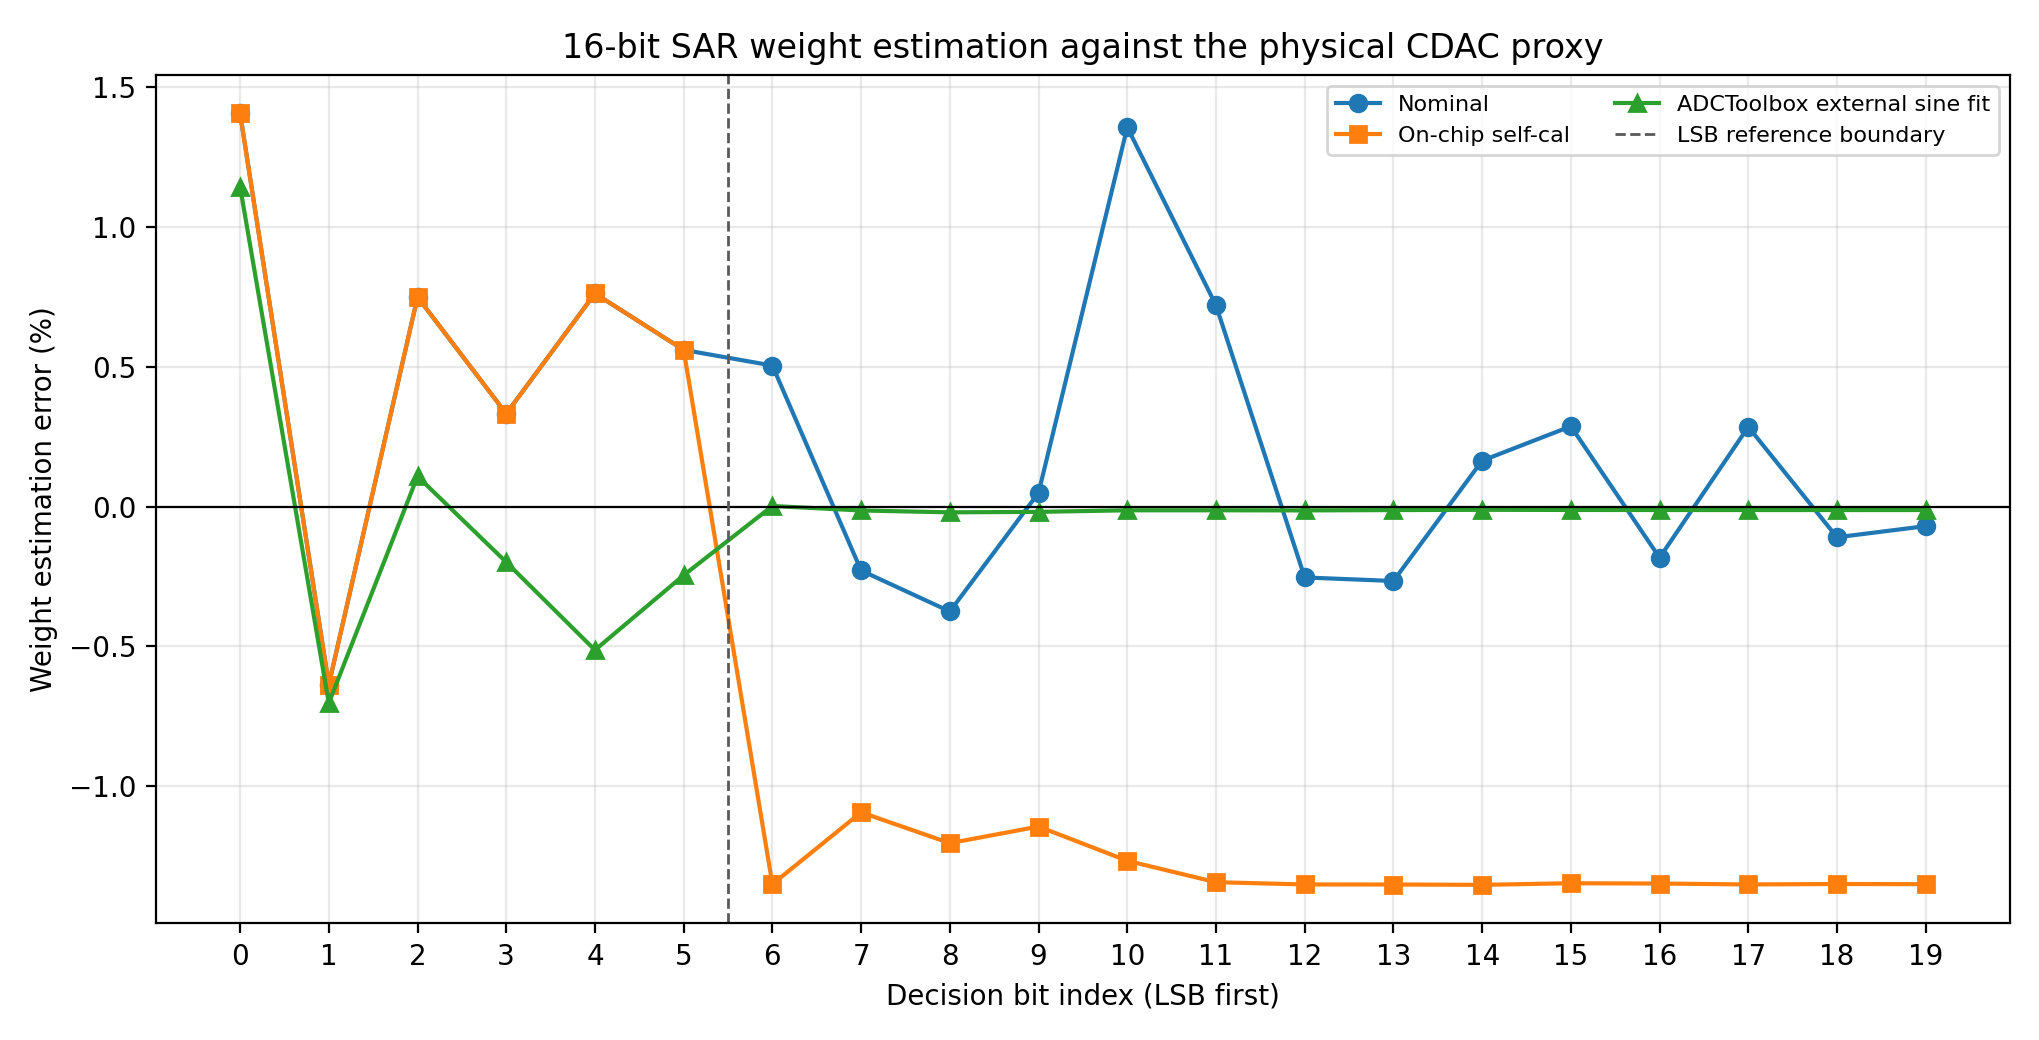
\includegraphics[width=0.94\textwidth]{fig_weight_error.png}
\caption{Nominal、片上自校准与外部 sine-fit 的逐权重误差。图中同时呈现 direct 与 gain-aligned 视角，防止把全局增益误判为相对非线性。}
\label{fig:weight-error}
\end{figure}

\begin{figure}[p]
\centering
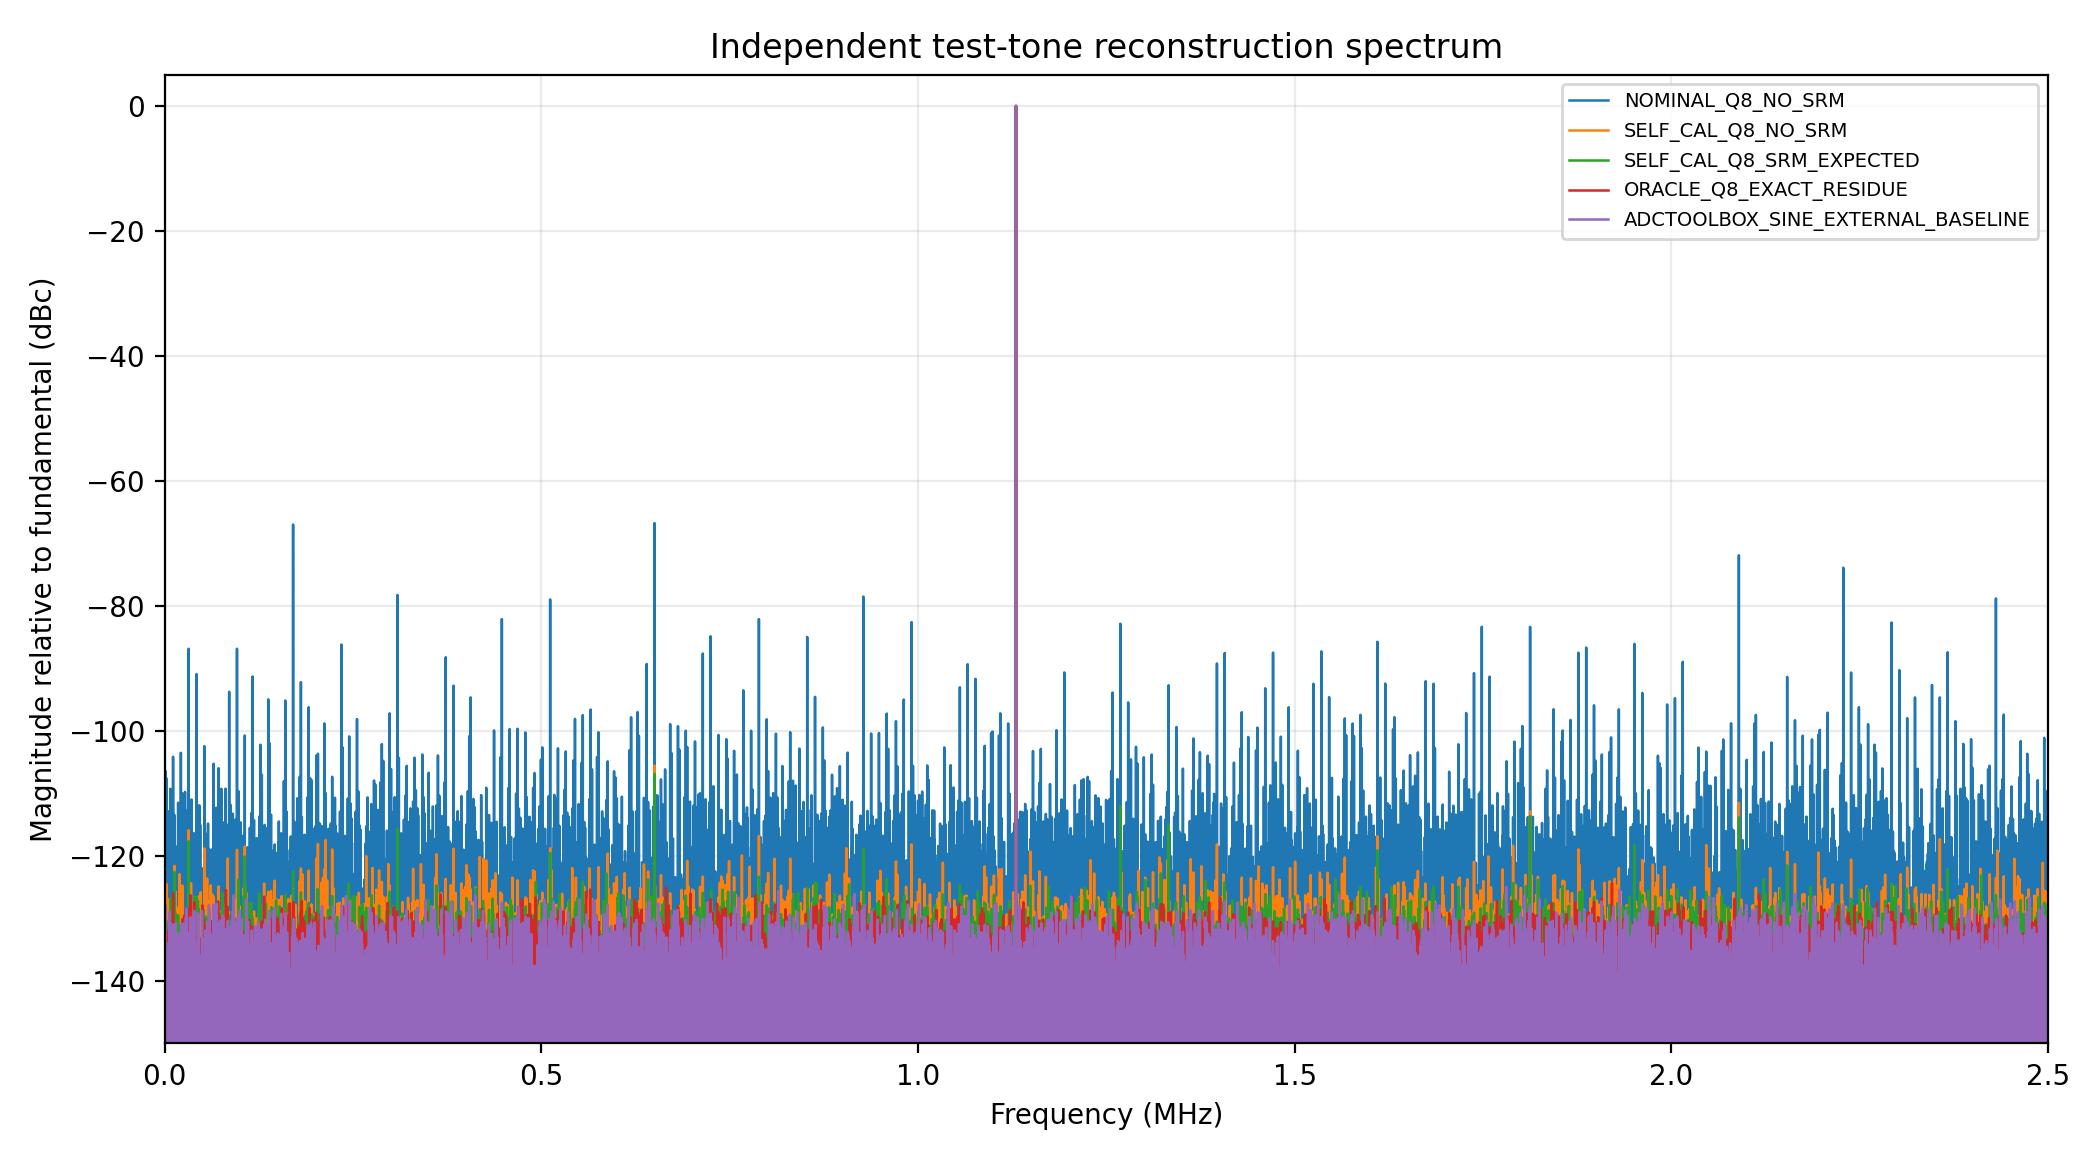
\includegraphics[width=0.96\textwidth]{fig_spectrum_compare.png}
\caption{独立 test-frequency capture 上的频谱对比。未校准失配产生强谐波；片上自校准显著恢复动态性能；oracle 与外部浮点拟合接近理想 16 位上限。}
\label{fig:spectrum}
\end{figure}

\begin{figure}[p]
\centering
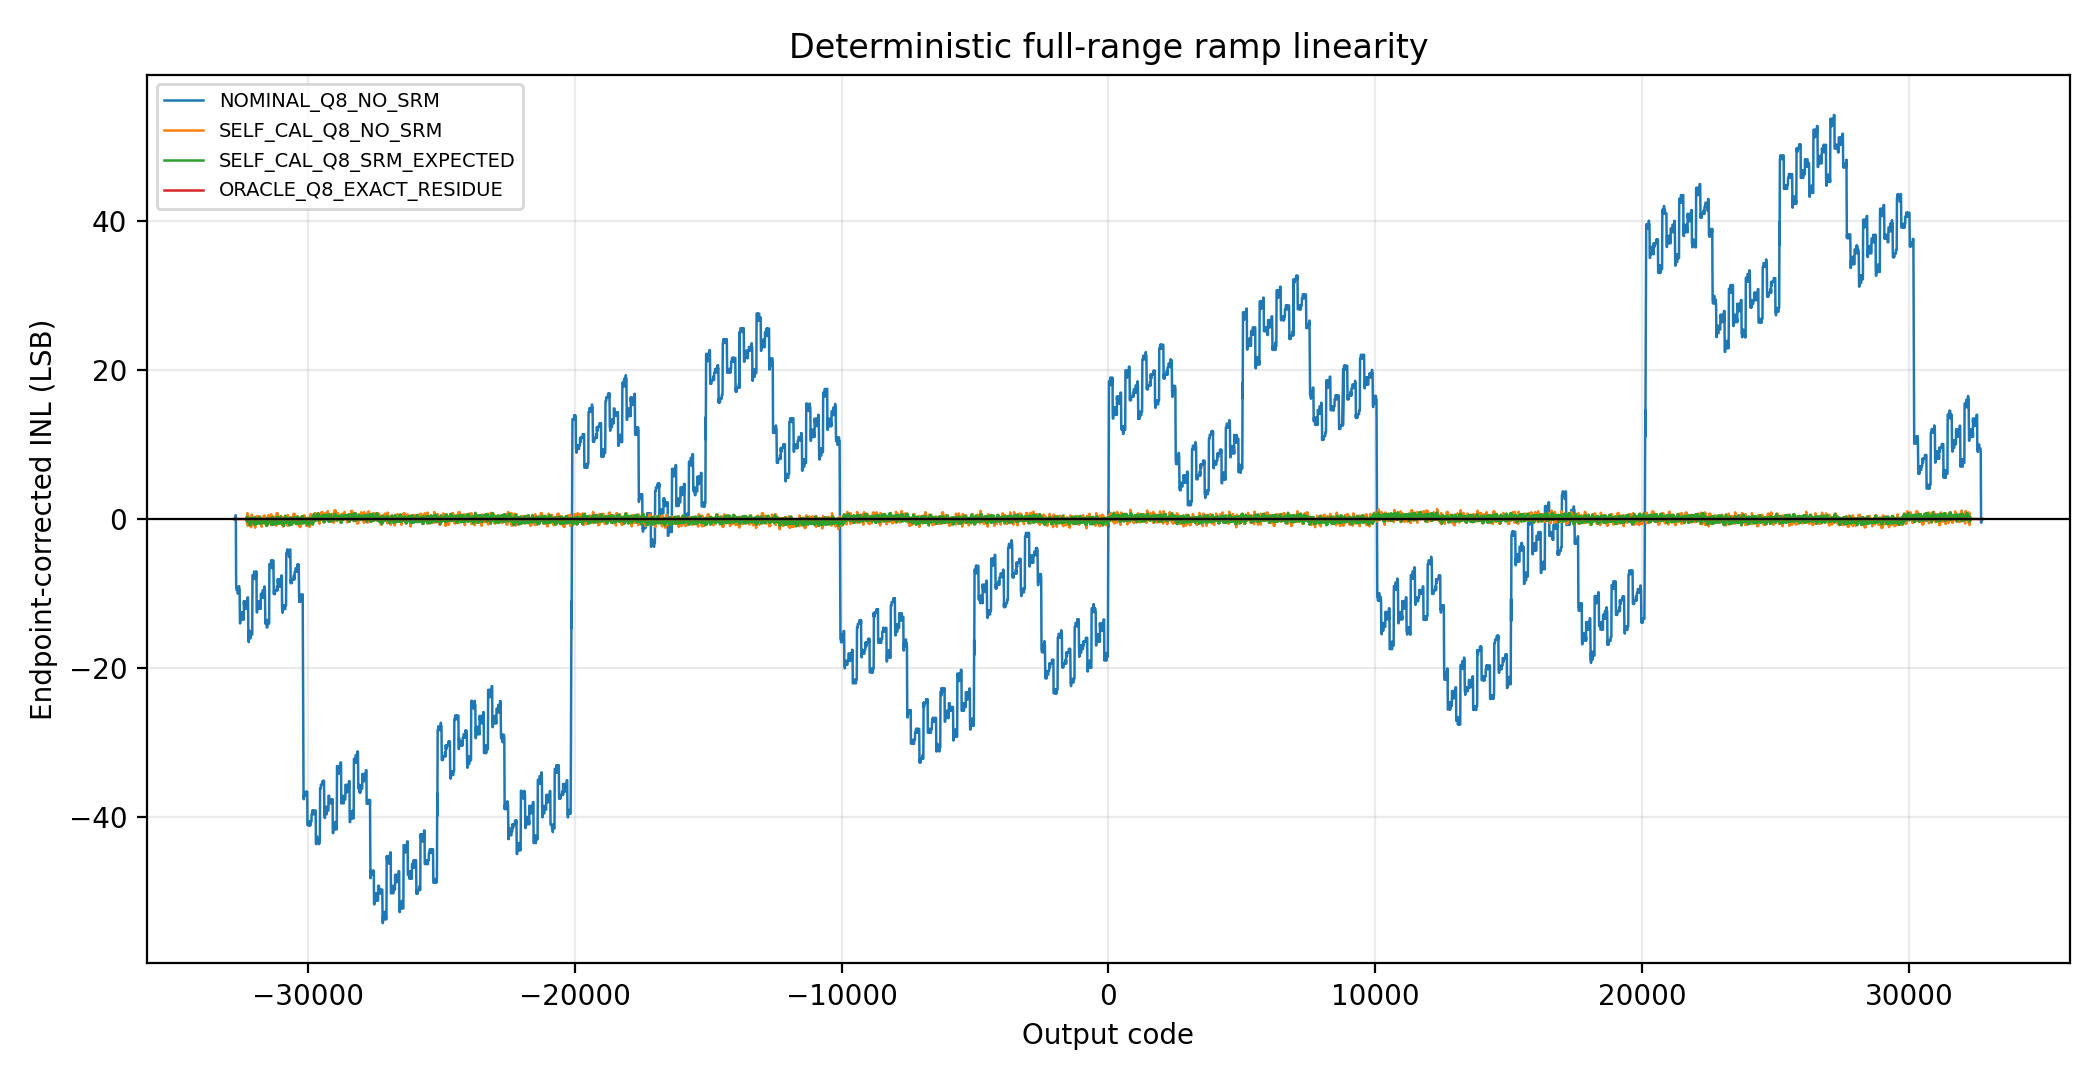
\includegraphics[width=0.96\textwidth]{fig_inl_compare.png}
\caption{Full-range ramp 的 endpoint-corrected INL 对比。片上校准将百 LSB 级失配台阶压缩到约 2 LSB 峰峰值。}
\label{fig:inl}
\end{figure}

\clearpage
\section{无噪声 residue-information 对照}

在 normal-path 随机噪声为 0 时，self-cal expected SRM 相对 no-SRM 增加 2.003 dB；22-decision stochastic case 相对 expected 上限损失 0.530 dB。这组结果说明 no-SRM 丢失了 segmented/redundant conversion 结束后的 analog residue information，而不是证明论文完整噪声抑制。

更关键的反证是 nominal weight path：
\begin{equation}
61.6297~\mathrm{dB}\ \text{(no SRM)}
\quad\text{vs}\quad
61.6319~\mathrm{dB}\ \text{(exact residue)}.
\end{equation}
仅差 0.0022 dB，说明错误 digital weights 才是未校准失真的主因；即便注入 exact residue，也无法修复几十 LSB 的权重台阶。

\section{带比较器噪声的 SRM 降噪结果}

\begin{table}[H]
\centering
\caption{共享 noisy raw bits 的 32-repeat SRM 成对消融}
\label{tab:srm-ablation}
\resizebox{\textwidth}{!}{%
\begin{tabular}{lrrrrr}
\toprule
Weight path & No SRM SNDR & 22-SRM SNDR & Paired gain & Error RMS no-SRM $\rightarrow$ SRM & Reduction\\
\midrule
Oracle physical & $90.532\pm0.054$ & $95.888\pm0.044$ & $5.356\pm0.056$ & $0.6203\rightarrow0.3348$ & $1.853\times$\\
Project self-cal & $89.716\pm0.059$ & $93.888\pm0.049$ & $4.172\pm0.079$ & $0.6722\rightarrow0.4158$ & $1.617\times$\\
\bottomrule
\end{tabular}}
\end{table}

Oracle expected-count noisy upper bound 为 $96.759\pm0.033$ dB。真实 22-count SRM 比 expected 上限低约 0.87 dB，但相对 no-SRM 仍有显著正收益。对 project self-cal weights，平均 SNDR 提升 4.17 dB，其方向和量级与论文中 SS 已开启时 $89.1\rightarrow93.7$ dB、约 4.6 dB 的趋势相近\cite{huang2025}。

\begin{evidencebox}{SRM 结论的准确边界}
该实验直接支持“22 次 noisy observations 的估计误差小于其消除的 comparator-decision/held-residue 误差”。它没有实现 split-sampling 的 $kT/C$ cancellation、AZ noise aliasing、前放带宽噪声谱或完整 reference path，因此只是机制与量级上的一致，不是论文硅片数值复现。
\end{evidencebox}

\begin{figure}[p]
\centering
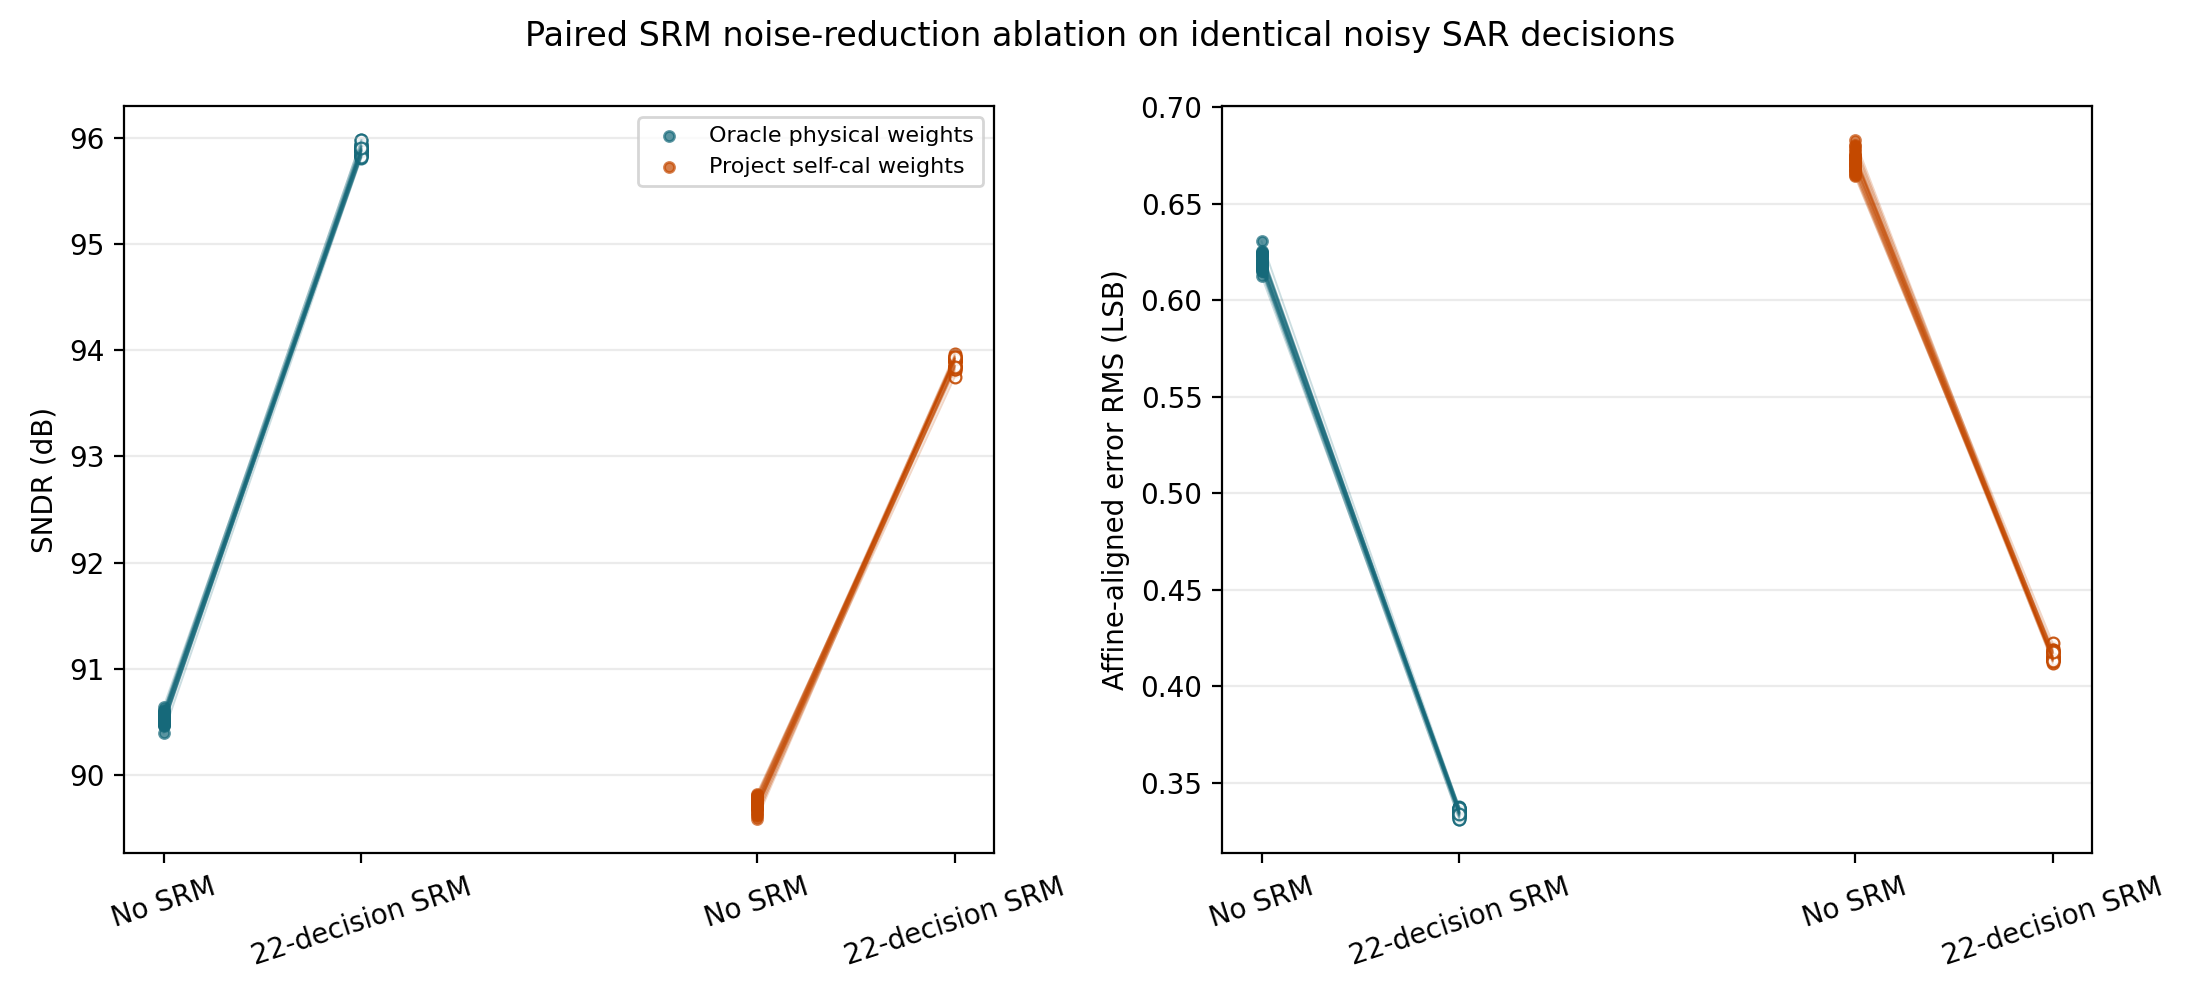
\includegraphics[width=0.97\textwidth]{fig_srm_noise_ablation.png}
\caption{SRM 公平成对带噪声消融。每个 repeat 内 on/off 共用同一 20-decision noisy raw-bit stream；连线展示 paired improvement。}
\label{fig:srm-ablation}
\end{figure}

\begin{figure}[p]
\centering
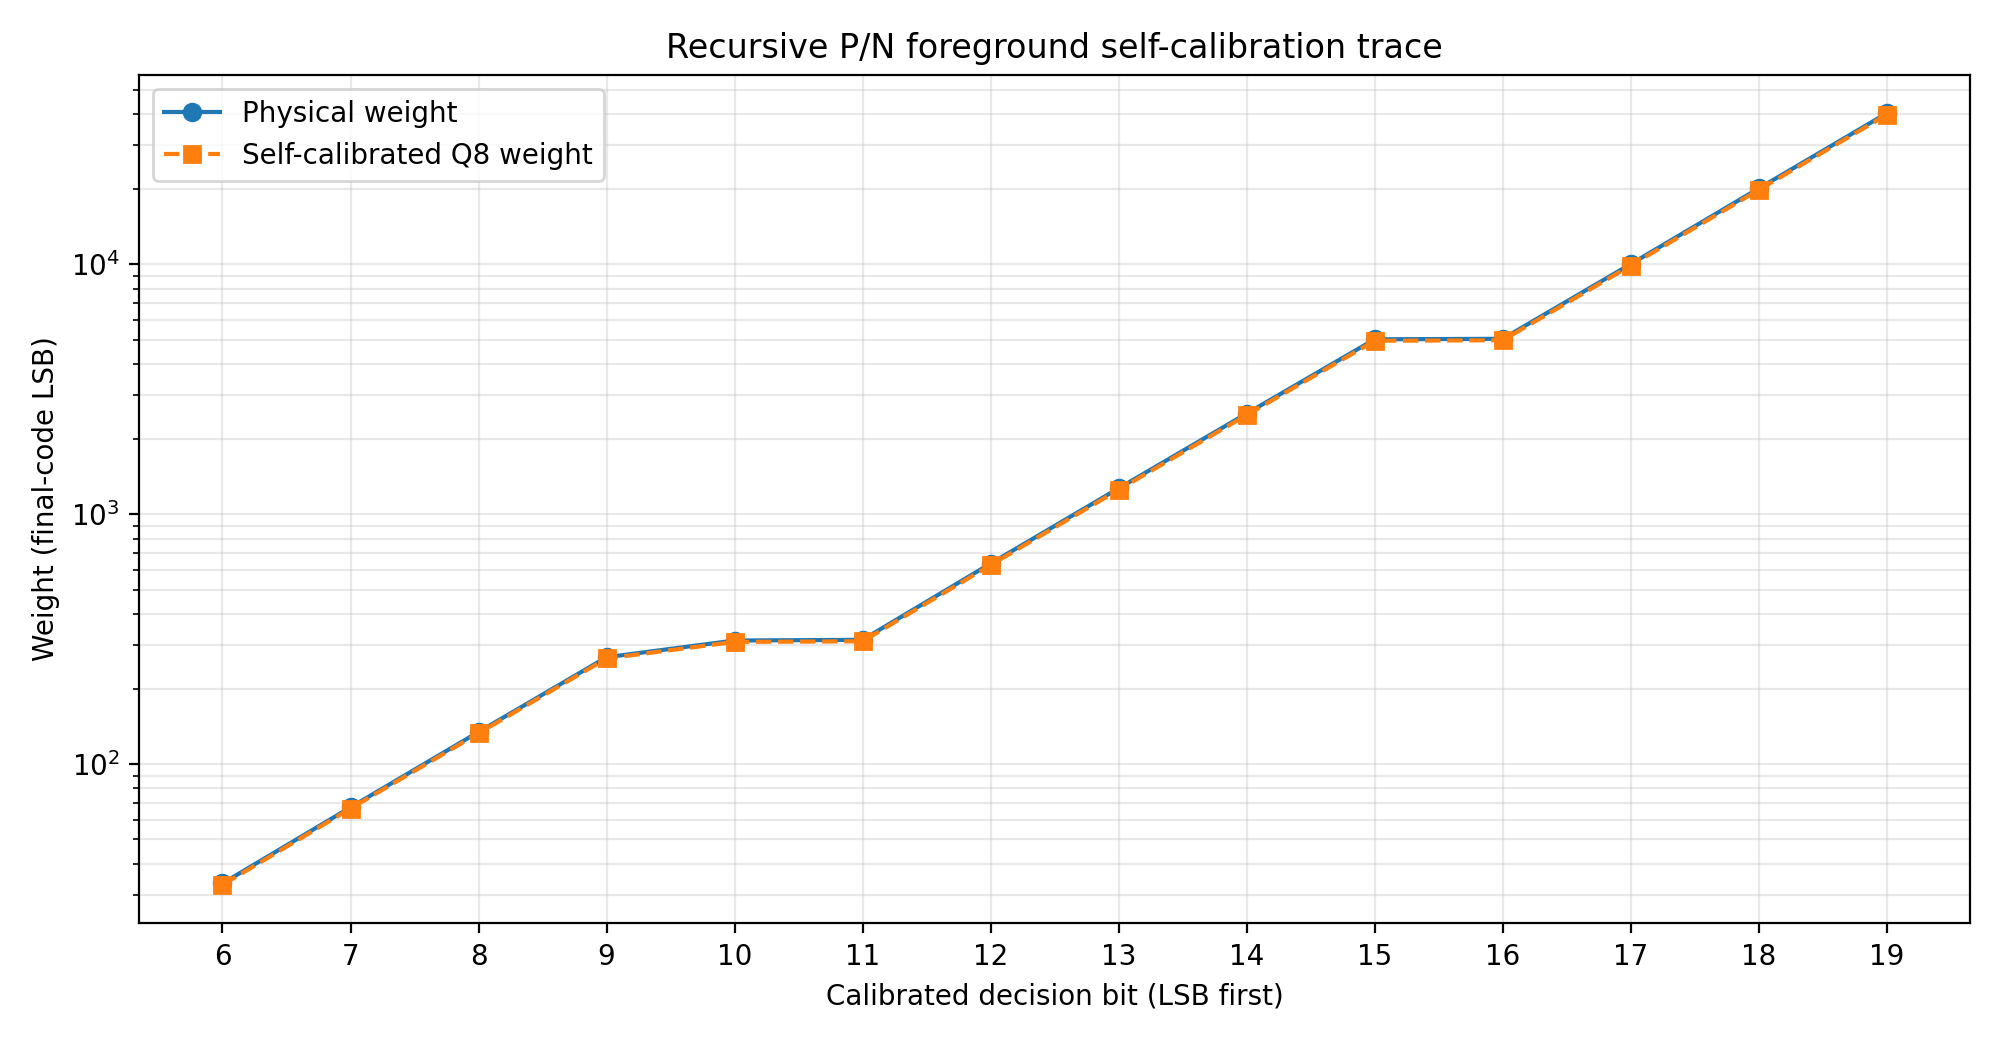
\includegraphics[width=0.96\textwidth]{fig_calibration_trace.png}
\caption{bit6 至 bit19 的递归校准轨迹。该图用于观察逐目标位估计、递归传播与最高两位保护，不等同于外部全局 least-squares fitting。}
\label{fig:cal-trace}
\end{figure}

\clearpage
\section{为什么结果会相差三十多 dB}

16 位线性度对大权重的相对误差极其敏感。本样本 effective-weight RMS relative mismatch 仅 0.5919\%，但按 final-code LSB 衡量，nominal 高 14 位 gain-aligned weight RMSE 达 11.099 LSB，最大误差 34.397 LSB，并形成约 108.5 LSBpp 的 INL 台阶。因此 SNDR 降到 61.63 dB 与量化理论并不矛盾。

Oracle weight no-SRM 为 95.1808 dB，expected SRM 后为 98.0205 dB，二者差 2.8397 dB，代表当前 segmented/redundant converter 的 residue-information gain。由 61.63 dB 到 95.18 dB 的大部分差距则来自 weight mismatch。片上自校准 no-SRM 相对 oracle no-SRM 尚差 1.7475 dB；expected SRM 后相对 oracle expected SRM 尚差 2.5837 dB，说明校准有效但并未达到 oracle 精度。

\section{512-chip 既有分布证据}

既有 512-chip revalidation 在其冻结配置下得到表\,\ref{tab:mc512}。它说明改善并非仅存在于 chip 17，但一个严重 outlier 的校准 SNDR 仅 55.619 dB，因此不能把均值或单颗提升解释为 silicon yield 保证。

\begin{table}[H]
\centering
\caption{既有 512-chip 行为级 revalidation 摘要}
\label{tab:mc512}
\begin{tabular}{lrrrr}
\toprule
Decoder & Mean/dB & Median/dB & P5/dB & P95/dB\\
\midrule
Nominal + SRM & 58.598 & 58.327 & 53.405 & 64.795\\
Current on-chip self-cal + SRM & 94.761 & 95.256 & 94.062 & 95.944\\
Oracle + SRM & 97.139 & 97.139 & 97.031 & 97.245\\
\bottomrule
\end{tabular}
\end{table}

% -----------------------------------------------------------------------------
\chapter{与 Huang 论文的联系、差异与复现距离}

\section{论文算法主线}

Huang 等的 16 位 split-sampling SAR ADC 使用 20 次冗余判决，并由 6-bit LSB DAC section 辅助测量 14 个高位权重；SS 与 SRM 用于降低 shorted-input noise、缩短 calibration averaging time，并在硅片上报告约 93.7 dB SNDR\cite{huang2025}。对应博士论文进一步讨论了该高分辨率信号链的时钟、采样与 SAR 设计背景\cite{huang2024}。

本项目与论文的联系在于：均以低 6 位参考高位权重；均需要前景自校准；均使用冗余 decision/reconstruction；均将 comparator/statistical information 用于 residue recovery。差异在于当前工程采用自己的 RTL 状态机、Q8 contract、P/N recursion、最高两位保护与 LUT，而不是从论文晶体管电路逐开关复制。

\section{已复现的数字边界}

\begin{table}[H]
\centering
\caption{论文相关功能的当前复现状态}
\label{tab:paper-distance}
\begin{tabularx}{\textwidth}{Xp{0.19\textwidth}X}
\toprule
功能 & 状态 & 当前证据\\
\midrule
6-bit LSB reference 测量 14 个高位权重 & 已实现 & 项目行为模型与 RTL interface\\
P/N polarity offset cancellation & 已实现 & 32-pair trace 与 5 LSB offset 条件\\
bit6--bit19 recursive update & 已实现 & per-target calibration trace\\
b18/b19 protection & 已实现 & 项目算法分支与行为回归\\
20-decision Q8 reconstruction & 已实现 & fixed-point decoder matrix\\
22-decision SRM count-to-Q8 & 已实现 & expected/stochastic 与 paired ablation\\
signed 16-bit saturation & 已实现 & ideal/full-range regression\\
VCM 首次切换和完整 analog switching & 未实现 & 需要 VM schematic/AMS 时序\\
SS/AZ 晶体管噪声机理 & 未实现 & 当前只隔离 comparator/residue 路径\\
论文硅片 93.7 dB 与功耗 & 未复现 & 需要 tapeout 或可信 PEX/AMS\\
\bottomrule
\end{tabularx}
\end{table}

\section{为什么论文 16 位实测可超过 94 dB}

理想 16 位量化极限约 98.08 dB。实测超过 94 dB 相当于 ENOB 约
\begin{equation}
\mathrm{ENOB}=\frac{94-1.76}{6.02}\approx15.32~\mathrm{bit},
\end{equation}
并不要求达到理想 16.00 bit，但要求总噪声、失配残差和动态失真均被压到约 0.7 bit 的综合预算内。论文通过 split sampling、SRM、低噪声前端、冗余和权重校准共同实现，而不是只靠数字权重修正。

本项目 ideal control 达到 98.093 dB；oracle expected-SRM 为 98.020 dB；project self-cal expected-SRM 为 95.437 dB。在行为模型范围内，该数字结果已越过 94 dB，但这并不自动证明真实电路会越过 94 dB，因为 VM 中还可能有采样热噪声、reference settling、switch nonlinearity、clock jitter、kickback、AZ aliasing 和带宽限制。

\begin{riskbox}{VCM 首次切换是待验证项}
当前行为模型未证明论文或 VM 电路中 normal conversion 开始前的首次 VCM/common-mode switching phase。若该相位遗漏，raw decision 的物理含义、residue polarity、comparator common mode 以及 P/N calibration stimulus 都可能改变。下一阶段必须从 SAR\_16B 原理图提取明确的 sample/VCM/first-trial/evaluate/hold 时序，并与 RTL transaction 对齐。
\end{riskbox}

\section{当前最准确的学术表述}

\begin{evidencebox}{推荐表述}
本工作完成了项目 16 位 SAR ADC 片上数字前景自校准算法及 SRM/Q8 重构边界的独立行为级闭环验证。结果表明，在 segmented physical-CDAC mismatch proxy 下，P/N 递归权重校准可显著降低失配引起的 INL 和动态失真；22-decision SRM 在共享 noisy raw-bit stream 的成对实验中进一步降低 comparator/residue error。真实 split-sampling、VCM switching、AZ、晶体管噪声、PEX 和硅片结果尚待验证。
\end{evidencebox}

% -----------------------------------------------------------------------------
\chapter{FPGA、ASIC 与流片风险审查}

\section{FPGA 可实施性}

三个核心 RTL 已有 Vivado 2018.3 综合和 XSIM 证据，行为模型也支持算法数值方向。当前仍需闭合：真实 top-level；raw-code atomic capture；EOC 与系统时钟 CDC；calibration/normal/SRM 三模式仲裁；\texttt{weights\_ready} 门控；同一 residue 的 transaction ownership；真实板级 XDC 与 I/O timing。

\begin{table}[H]
\centering
\caption{FPGA 集成检查表}
\label{tab:fpga-risks}
\begin{tabularx}{\textwidth}{p{0.27\textwidth}p{0.16\textwidth}X}
\toprule
项目 & 当前状态 & 关闭条件\\
\midrule
核心 RTL 可综合 & 已有证据 & 在目标器件/时钟重新执行 synth/impl 与 timing report\\
权重写回原子性 & 待闭合 & 双缓冲或明确 conversion idle write window\\
\texttt{weights\_ready} & 待闭合 & 校准完成前禁止 normal reconstruction\\
CDC/RDC & 待闭合 & EOC、start、done、comparator path 完成结构审查和约束\\
SRM residue ownership & 待闭合 & 22 次观察必须属于同一 conversion-held residue\\
XDC & 部分 & 核心 timing 与 legacy board hints 分离\\
\bottomrule
\end{tabularx}
\end{table}

\section{ASIC 实现风险}

\begin{table}[H]
\centering
\small
\caption{RTL 到 GDS 的关键风险}
\label{tab:asic-risks}
\begin{tabularx}{\textwidth}{L{0.20\textwidth}L{0.27\textwidth}Y}
\toprule
领域 & 风险 & 必需验证\\
\midrule
Calibration PHY & \path{dac_p_force/dac_n_force} 仍为抽象控制 & 明确 switch-level sequencer、VCM phase、reset/AZ/evaluate/READYN timing\\
数值与溢出 & Q8 register、accumulator、负数 rounding 与 saturation & formal properties、corner vectors、GLS/X-propagation\\
时序与 CDC & analog EOC/comparator 与 digital clock 边界 & CDC/RDC、synchronizer/handshake、SDC exception review\\
PVT 与噪声 & 32-pair 平均假设可能受相关噪声和 bias 破坏 & AMS PVT/MC、noise spectrum、reference settling sweep\\
功耗与时间 & 14 targets $\times$ 32 P/N pairs + 22 SRM decisions & calibration latency、energy、timeout 与 duty-cycle budget\\
可测性 & 内部权重、状态、residue 不可见 & scan/MBIST、calibration readback、silicon debug mux\\
Physical design & 约束、时钟、复位、拥塞与 IR drop & MMMC、LEC、DFT、PnR、STA、EM/IR\\
Signoff & 版图寄生改变 CDAC/clock/control & DRC/LVS/PEX、post-layout AMS 与数字 GLS\\
\bottomrule
\end{tabularx}
\end{table}

\section{三轮独立全流程审查结论}

\begin{enumerate}
  \item \textbf{算法层审查：}固定点、P/N 估计、递归、保护、SRM 与 decoder matrix 一致；失配和噪声问题已分实验回答。
  \item \textbf{实现层审查：}RTL 核心可作为数字算法核，但缺完整 calibration PHY、top、CDC 与 transaction control；不能直接接入真实 SAR\_16B 电路而不做 adapter。
  \item \textbf{流片层审查：}当前无 SDC/MMMC、LEC、DFT、PnR、DRC/LVS/PEX 与 post-layout AMS 证据，因此只可作为 architecture/behavior baseline，不能称为 tapeout-ready。
\end{enumerate}

\begin{diagnosticbox}{潜在论文创新空间}
相对于仅做离线权重拟合，较有价值的方向包括：低开销 P/N 递归校准与 top-bit protection 的形式化误差界；SRM 与权重校准共用 comparator/statistical engine；VCM/split-sampling 时序与数字 transaction co-design；基于在线 residue statistics 的自适应 averaging/early-stop；以及 Q8 精度、校准能耗、收敛时间和高位失配容限之间的可测 Pareto。任何 TCAS/JSSC 主张都需由 AMS/PEX/硅片证据支持。
\end{diagnosticbox}

% -----------------------------------------------------------------------------
\chapter{可复现性、维护与交付}

\section{冻结运行命令}

\begin{reproductionbox}{Windows PowerShell 复现}
\begin{lstlisting}
$py = "C:\Users\Administrator\Desktop\ADCToolbox_EVAL_20260728\envs\upstream-main\Scripts\python.exe"

& $py -m py_compile `
  analysis\self_cal_adctoolbox_behavioral_20260830\run_self_cal_behavioral.py `
  analysis\self_cal_adctoolbox_behavioral_20260830\test_self_cal_behavioral.py

& $py -m pytest `
  analysis\self_cal_adctoolbox_behavioral_20260830\test_self_cal_behavioral.py -q

& $py `
  analysis\self_cal_adctoolbox_behavioral_20260830\run_self_cal_behavioral.py
\end{lstlisting}
\end{reproductionbox}

\section{结果追溯规则}

\begin{enumerate}
  \item 性能数字优先引用 \texttt{outputs/summary.json}；逐 decoder 表引用 \texttt{metrics.csv}。
  \item SRM 统计分布引用 \texttt{srm\_noise\_ablation.csv}，并同时写明 repeat count 与 noise conditions。
  \item 权重结论必须区分 direct 与 gain-aligned RMSE，并记录 alignment factor。
  \item 所有图均由上述结构化数据生成；图不是唯一证据源。
  \item 重新运行时必须记录 Python、NumPy、Matplotlib、ADCToolbox 版本与 toolbox commit。
  \item 若修改核心 RTL，必须同步更新行为模型、fixed-point contract、TB 与本报告结果。
\end{enumerate}

\section{维护建议}

后续建议将验证分为四条稳定流水线：
\begin{enumerate}
  \item \textbf{Fast contract CI：}py\_compile、unit tests、固定 seed 的 ideal/mismatch smoke；
  \item \textbf{Numerical regression：}16384-point FFT、131072-point ramp、expected/stochastic SRM；
  \item \textbf{Statistical regression：}32-repeat paired noise ablation 与 512-chip mismatch sweep；
  \item \textbf{EDA regression：}Vivado XSIM/synthesis，随后扩展 AMS、CDC、STA 与 physical signoff。
\end{enumerate}

\begin{riskbox}{版本维护纪律}
行为输出、报告和核心 RTL 必须绑定同一 Git 提交。任何删除都先归档；外部工具箱版本必须固定到 commit；不要在报告中只写“最新版本”。当算法 contract 改变时，应提升 \texttt{summary.json} schema version 并使旧结果仍可追溯。
\end{riskbox}

% -----------------------------------------------------------------------------
\chapter{结论}

\begin{enumerate}
  \item \textbf{16 位定义：\statuspass。}最终输出是 signed 16 bit；20 仅是冗余判决数。
  \item \textbf{片上自校准身份：\statuspass。}主模型执行 6-bit reference、P/N、32 pairs、bit6--bit19 recursion、top-bit protection 和 Q8 writeback。
  \item \textbf{理想基准：\statuspass。}98.093 dB 与 16 位理论 98.080 dB 对齐。
  \item \textbf{失配校准有效性：\statuspass。}同一 physical sample 中 SNDR 提升 31.804 dB，gain-aligned weight RMSE 改善 40.63 倍。
  \item \textbf{SRM 数字行为：\statuspass。}同一 noisy raw-bit stream 上，22-decision SRM 使 oracle/self-cal 平均 SNDR 分别提高 5.356/4.172 dB。
  \item \textbf{ADCToolbox 角色：\statuspass。}已验证为分析工具与外部 baseline，不属于片上算法。
  \item \textbf{FPGA/ASIC 集成：\statusgap。}adapter、CDC、mode arbiter、calibration PHY 和真实 VCM 时序尚未闭合。
  \item \textbf{GDS/硅片：\statusnoclaim。}本报告没有把行为结果升级为 tapeout 或 measured-silicon 结论。
\end{enumerate}

\begin{passbox}{最终工程判断}
当前项目的 16 位片上前景自校准数字算法在行为级 physical-CDAC mismatch 模型中确实有效；当前 SRM 数字行为模型也在公平成对带噪声实验中显示明确降噪收益。两者已通过理想 16 位锚点、独立 test frequency、full-range ramp、expected/stochastic SRM、paired noisy ablation 与外部 toolbox baseline 的多重交叉验证。下一步应优先闭合 SAR\_16B VM 原理图的 VCM/CDAC/comparator 时序与 AMS 噪声预算，再进入 CDC、ASIC 与 physical signoff。
\end{passbox}

% -----------------------------------------------------------------------------
\appendix
\chapter{输出文件与字段索引}

\begin{longtable}{L{0.35\textwidth}L{0.54\textwidth}}
\caption{交付文件用途}\label{tab:output-index}\\
\toprule
文件 & 用途\\
\midrule
\endfirsthead
\toprule
文件 & 用途\\
\midrule
\endhead
\path{outputs/summary.json} & 配置、版本、mismatch realization、ideal control、decoder metrics、SRM ablation summary 与 evidence boundary\\
\path{outputs/metrics.csv} & 所有 decoder 的 SNDR/SNR/SFDR/THD/ENOB、DNL/INL 与 missing-code 汇总\\
\path{outputs/weights.csv} & nominal、physical truth、self-cal、external fit 的逐 bit 权重与误差\\
\path{outputs/srm_noise_ablation.csv} & 32 repeats $\times$ 5 decoders 的逐次动态指标与 aligned error RMS\\
\path{outputs/calibration_trace.json} & bit6--bit19 的 P/N measurement、递归更新和 protection trace\\
\path{outputs/run_log.txt} & 最终完整实验 stdout\\
\path{outputs/fig_weight_error.png} & 权重误差图\\
\path{outputs/fig_spectrum_compare.png} & 独立测试频率频谱图\\
\path{outputs/fig_inl_compare.png} & Full-range ramp INL 图\\
\path{outputs/fig_calibration_trace.png} & 递归校准轨迹图\\
\path{outputs/fig_srm_noise_ablation.png} & SRM 成对带噪声消融图\\
\bottomrule
\end{longtable}

\chapter{复核清单}

\begin{table}[H]
\centering
\caption{独立复核者应执行的最小清单}
\label{tab:review-checklist}
\begin{tabularx}{\textwidth}{p{0.08\textwidth}X p{0.16\textwidth}}
\toprule
序号 & 检查内容 & 预期\\
\midrule
1 & 确认输出 16 bit、raw decisions 20、Q8 中 256 = 1 LSB & 一致\\
2 & 运行 ideal direct quantizer & SNDR 约 98.09 dB\\
3 & 对同一 chip 比较 nominal/self-cal weights & aligned RMSE 显著下降\\
4 & 对同一 raw bits 比较 SRM off/on & raw bits identity 为 true\\
5 & 检查 noisy ablation 的 paired SNDR gain & oracle/self-cal 均为正\\
6 & 检查 full-range ramp & self-cal missing code 4；expected SRM 为 0\\
7 & 检查 external sine fit 的命名和矩阵形状 & 明确 external；$N\times20$\\
8 & 检查报告中的证据边界 & 不出现 PEX、GDS 或硅片过度声明\\
\bottomrule
\end{tabularx}
\end{table}

\chapter{术语与缩写}

\begin{longtable}{L{0.19\textwidth}L{0.70\textwidth}}
\toprule
缩写 & 含义\\
\midrule
\endfirsthead
\toprule
缩写 & 含义\\
\midrule
\endhead
SAR & Successive Approximation Register\\
CDAC & Capacitive Digital-to-Analog Converter\\
SRM & Statistical Residue Measurement\\
SS & Split Sampling\\
AZ & Auto-Zero\\
Q8 & 具有 8 个小数位的 signed fixed-point 表示\\
SNDR & Signal-to-Noise-and-Distortion Ratio\\
SFDR & Spurious-Free Dynamic Range\\
INL/DNL & Integral/Differential Nonlinearity\\
CDC/RDC & Clock/Reset Domain Crossing\\
AMS & Analog/Mixed-Signal simulation\\
PEX & Parasitic Extraction\\
LEC & Logical Equivalence Checking\\
MMMC & Multi-Mode Multi-Corner analysis\\
\bottomrule
\end{longtable}

\clearpage
\begin{thebibliography}{9}

\bibitem{huang2025}
Q. Huang et al., ``A 5-MS/s 16-bit Low-Noise and Low-Power Split Sampling SAR ADC With Eased Driving Burden,'' \emph{IEEE Journal of Solid-State Circuits}, 2025. 工程本地 Zotero 证据副本已冻结。

\bibitem{huang2024}
Q. Huang, \emph{Advanced Clock Multiplier and SAR ADC Design Techniques for High-Resolution Signal Chain Systems}, doctoral dissertation, 2024. 工程本地 Zotero 证据副本已冻结。

\bibitem{adctoolbox}
Arcadia Labs, \emph{ADCToolbox}, version 0.9.1, reviewed commit \texttt{a8995cf4faf7} (full hash in Table~\ref{tab:doc-control}). Used in this report for characterization metrics and an explicitly external sine-fit baseline.

\bibitem{projectmodel}
SAR ADC Digital Process Project, \emph{Full SAR Behavioral Model, Physical CDAC Mismatch Model, and Core RTL}, evidence commit \texttt{\EvidenceCommit}, 2026.

\end{thebibliography}

\clearpage
\thispagestyle{empty}
\vspace*{0.22\textheight}
\begin{center}
{\ReferenceCJKTitle\bfseries\fontsize{17.22}{27}\selectfont 报告结束}\par
\vspace{0.8cm}
{\color{RefNavy}\rule{0.18\textwidth}{1.0pt}}\par
\vspace{1.0cm}
\begin{tabular}{rl}
\textbf{工程：} & SAR ADC Digital Process\\
\textbf{证据提交：} & \texttt{\EvidenceCommit}\\
\textbf{报告源：} & \texttt{SAR16B\_SELF\_CAL\_SRM\_BEHAVIORAL\_REPORT\_CN.tex}\\
\textbf{构建器：} & XeLaTeX\\
\textbf{日期：} & 2026-08-30\\
\end{tabular}
\vfill
{\small 行为级结果须与其条件、decoder 和证据边界共同引用。}
\end{center}

\end{document}
